\documentclass[11pt]{article}

\usepackage{url}
%\usepackage[margin=2.5cm]{geometry} % See geometry.pdf to learn the layout options. There are lots.
\usepackage{geometry}
\geometry{a4paper} %or letterpaper or a5paper or ...

%for figures and graphics
\usepackage{graphicx}
\usepackage{subcaption} %allows subfigures
\usepackage[bottom]{footmisc} %footnotes go below figures
%\usepackage{parskip} %adds line space between paragraphs by default

\DeclareGraphicsRule{.tif}{png}{.png}{`convert #1 `dirname #1`/`basename #1 .tif`.png}
\graphicspath{{../Diagrams/Diagram_PDFs/} {../Diagrams/Numerical_Results/}}

%\input imports all commands from the target files
%The idea behind this file is that it will be used to store all the maths-related macros that I concoct; so that I can import all the commands by \input{this file} in the preamble of any file that I want to use them in.
%This should make the top-level files look a lot cleaner, and the preamble much shorter!

\usepackage{amssymb}
\usepackage{amsmath}
%\usepackage{mathtools}

%theorems and lemma etc setup using amsthm
\usepackage{amsthm}
\theoremstyle{definition}
\newtheorem{definition}{Definition}[section]
\theoremstyle{plain}
\newtheorem{theorem}{Theorem}[section]
\theoremstyle{plain}
\newtheorem{lemma}[theorem]{Lemma}
\theoremstyle{plain}
\newtheorem{prop}[theorem]{Proposition}
\theoremstyle{plain}
\newtheorem{cory}[theorem]{Corollary}
\theoremstyle{definition}
\newtheorem{convention}[theorem]{Convention}
\theoremstyle{definition}
\newtheorem{assumption}[theorem]{Assumption}
\theoremstyle{definition}
\newtheorem{conjecture}[theorem]{Conjecture}

\allowdisplaybreaks %allows equations in the same align environment to split over multiple pages.

%tstk always need be there
\newcommand{\tstk}[1]{\textbf{#1} \newline}

%this adds extra functionality to pmatrix, vmatrix, bmatrix etc by allowing you to pass an optional argument in [FACTOR] to multiply the default spacing between elements by FACTOR
\makeatletter
\renewcommand*\env@matrix[1][\arraystretch]{%
  \edef\arraystretch{#1}%
  \hskip -\arraycolsep
  \let\@ifnextchar\new@ifnextchar
  \array{*\c@MaxMatrixCols c}
  }
\makeatother

%begin the macros via newcommand. Try to group them up reasonably!

%notation and variable use throughout the file
\renewcommand{\vec}[1]{\mathbf{#1}}				%vectors are bold, not overline arrow
\newcommand{\recip}[1]{\frac{1}{#1}}			%fast reciprocal as a fraction
\newcommand{\interval}[1]{\sqbracs{0,\abs{#1}}}	%creates the closed interval from 0 to the length of the input #1, denoted by absolute value
\newcommand{\eps}{\varepsilon}					%pretty epsilons
\newcommand{\charFunc}[1]{\mathcal{I}_{#1}}%{\mathbb{1}_{#1}}		%characteristic function of a set

\newcommand{\dddom}{\widetilde{\Omega}}			%3D domain notation
\newcommand{\ddom}{\Omega}						%2D domain notation
\newcommand{\dddmes}{\widetilde{\mu}}			%3D measure
\newcommand{\ddmes}{\mu}						%2D measure

\newcommand{\graph}{\mathbb{G}}					%graph variable
\newcommand{\vertSet}{\mathcal{V}}					%set of vertices rather than big V
\newcommand{\edgeSet}{\mathcal{E}}					%set of edges rather than large E, \graph = (V,E)
\newcommand{\wavenumber}{\kappa}				%fourier variable or wavenumber, not to confuse with jk subscripts!
\newcommand{\qm}{\theta}						%quasi-momentum parameter
\newcommand{\kt}{\bracs{\wavenumber, \qm}}		%(k, theta) pair
\newcommand{\dmap}{\Gamma_0}					%Dirichlet map
\newcommand{\nmap}{\Gamma_1}					%Neumann map
\newcommand{\effFreq}{\Lambda}					%Effective frequency sqrt(w^2-\wavenumber^2)
\newcommand{\conLeft}{\stackrel{\rightarrow}{\smash{\sim}\rule{0pt}{0.4ex}}} %j connects to k, j left
\newcommand{\conRight}{\stackrel{\leftarrow}{\smash{\sim}\rule{0pt}{0.4ex}}} %j connects to k, j right
\newcommand{\con}{\sim}							%j connects to k, indifferent of direction

%standard sets
\newcommand{\naturals}{\mathbb{N}}			%natural numbers
\newcommand{\integers}{\mathbb{Z}}			%integers
\newcommand{\rationals}{\mathbb{Q}}			%rational numbers
\newcommand{\reals}{\mathbb{R}}				%real numbers
\newcommand{\complex}{\mathbb{C}}			%complex numbers

%brackets and norms
\newcommand{\bracs}[1]{\left( #1 \right)}				%encloses input in brackets
\newcommand{\sqbracs}[1]{\left[ #1 \right]}				%encloses input in square brackets
\newcommand{\clbracs}[1]{\left\{ #1 \right\}}			%encloses input in curly bracers
\newcommand{\abs}[1]{\left\lvert #1 \right\rvert}					%absolute value
\newcommand{\norm}[1]{\lvert\lvert #1 \rvert\rvert}		%norm 

%function sets
\newcommand{\smooth}[1]{C^{\infty}\bracs{#1}}							%smooth functions
\newcommand{\ltwo}[2]{L^{2}\bracs{#1,\mathrm{d}#2}}						%general L^2 space
\newcommand{\gradSob}[2]{H^1_\mathrm{grad}\bracs{#1, \mathrm{d}#2}}		%gradient Sobolev space
\newcommand{\gradSobQM}[2]{H^1_{\qm, \mathrm{grad}}\bracs{#1, \mathrm{d}#2}} %gradient + i\qm Sobolev space
\newcommand{\ktgradSob}[2]{H^1_{\wavenumber,\qm,\mathrm{grad}}\bracs{#1, \mathrm{d}#2}}	%k,\qm-gradient Sobolev space
\newcommand{\curlSob}[2]{H^1_\mathrm{curl}\bracs{#1, \mathrm{d}#2}}		%curl Sobolev space
\newcommand{\tcurlSob}[2]{H^1_{\qm, \mathrm{curl}}\bracs{#1, \mathrm{d}#2}}		%curl + i\qm Sobolev space
\newcommand{\kcurlSob}[2]{H^1_{\wavenumber,\mathrm{curl}}\bracs{#1, \mathrm{d}#2}}	%k-curl Sobolev space
\newcommand{\ktcurlSob}[2]{H^1_{\wavenumber,\qm,\mathrm{curl}}\bracs{#1, \mathrm{d}#2}}	%k,\qm-curl Sobolev space
\newcommand{\ktcurlSobDivFree}[2]{\mathcal{H}^{\kt}\bracs{#1, \mathrm{d}#2}}					%k,\qm-curl, divergence-free Sobolev space
\newcommand{\supp}{\mathrm{supp}}										%support of a function

%grad and curl sets
\newcommand{\gradZero}[2]{\mathcal{G}_{ #1, \mathrm{d}#2}\bracs{0}}		%gradients of zero for domain #1 with measure #2
\newcommand{\kgradZero}[2]{\mathcal{G}_{ #1, \mathrm{d}#2}^{(\wavenumber)}\bracs{0}}	%k-gradients of zero for domain #1 with measure #2
\newcommand{\curlZero}[2]{\mathcal{C}_{ #1, \mathrm{d}#2}\bracs{0}}	%curls of zero for domain #1 with measure #2
\newcommand{\kcurlZero}[2]{\mathcal{C}_{ #1, \mathrm{d}#2}^{(\wavenumber)}\bracs{0}}	%k-curls of zero for domain #1 with measure #2

%derivatives and grad-like symbols
\newcommand{\diff}[2]{\dfrac{\mathrm{d}#1}{\mathrm{d}#2}}			%complete derivative d#1/d#2
\newcommand{\pdiff}[2]{\dfrac{\partial #1}{\partial #2}}			%partial derivative p#1/p#2
\newcommand{\ddiff}[2]{\dfrac{\mathrm{d}^2 #1}{\mathrm{d} {#2}^2}}	%2nd deriv
\newcommand{\grad}{\nabla}											%grad operator
\newcommand{\tgrad}{\nabla^{\qm}}									%grad operator with qm superscript
\newcommand{\kgrad}{\grad^{(\wavenumber)}}							%grad with wavenumber superscript
\newcommand{\ktgrad}{\grad^{\kt}}				%grad with wavenumber, qm superscript
\newcommand{\curl}[1]{\grad_{#1}\wedge}							%curl with subscript #1
\newcommand{\kcurl}[1]{\grad_{#1}^{(\wavenumber)}\wedge}			%k-curl with measure subscript #1
\newcommand{\ktcurl}[1]{\grad_{#1}^{\kt}\wedge}		%k,theta-curl with measure subscript #1
\newcommand{\laplacian}{\Delta}						%laplacian operator, can have subscripts attached

%displaying integrals
\newcommand{\integral}[3]{\int_{#1}#2 \ \mathrm{d}#3}			%integral, domain #1, integrand #2, measure #3
\newcommand{\md}{\mathrm{d}}									%differential d

%convergence
%\newcommand{\lconv}[1]{\xrightarrow{#1}}							%convergence with #1 above the rightarrow - requires mathtools
\newcommand{\lconv}[1]{\overset{#1}{\longrightarrow}}				%convergence with #1 above the rightarrow
\newcommand{\toInfty}[1]{ \ \text{as} \ #1 \rightarrow\infty}		%writes out "as #1 tends to infty" %maths commands, variables, and other packages

%labelling hacks
\newcommand\labelthis{\addtocounter{equation}{1}\tag{\theequation}}

%reminders of things to fill in
%\newcommand{\tstk}[1]{\textbf{#1}\newline}

%changes the title of the bibliography page to ``References"
\renewcommand{\refname}{References} %NB: For reports, this is \bibname rather than \refname

\title{Paper Title}  % Declares the document's title.
\author{Authors} 	% Declares the author's name.
\date{\today}      % commenting out this command produces today's date.

%-------------------------------------------------------------------------
%DOCUMENT STARTS

\begin{document}


%REPORT BEGINS

\maketitle

%\input chapters one at a time; the references should all match up and can even cross-reference; however you won't get prompts for references across files when editing.
%NB: Can use \include for speed, but then the directory fills up with useless .aux files.
%To save time, comment out sections that aren't being edited. References may disappear but the file will still compile!

\begin{abstract}

We develop a mathematical framework for the study of wave propagation in two-dimensional photonic crystals whose cross-sections are well approximated by ``graph-like" structures. 
We study spectral properties of such structures for various types of coupling conditions at the junctions between the graph edges, in the case of transverse polarisation, when either the electric or magnetic field is aligned with the crystal.

\end{abstract}

\section{Introduction} \label{sec:Intro}

\tstk{This section includes our literature review and motivation.
The purpose of the paper is to present the equations that were derived for the TFR/curl-curl system as what can be interpreted as an "effective" or "limit" problem for a fine/thin-structure material.
This is subject to future advances in the field that draw parallel to the scalar-case developments, of course.
This text should be deleted upon completion of the LitReview.}

\subsection{Lit Review} \label{ssec:LitReview}

\subsection{Physical Motivation} \label{ssec:PhysMot}
The problem we consider in this work is motivated by the desire to study wave propagation in a medium that exhibits a periodic (micro)-structure.
Understanding the behaviour of waves in such media has applications in the field of photonic crystals, but also extends broadly into the study of wave behaviour in an elastic setting too (see section \ref{ssec:LitReview}), although our motivations largely stem from the former.
One starting point for the study of such phenomena is the wave equation;
\begin{align} \label{eq:DimensionalWaveEqn}
	-A \laplacian u &= f^2 \rho u,
\end{align}
where $f$ is understood as the frequency of a propagating wave, with $A$ and $\rho$ representing physical properties of the medium that \eqref{eq:DimensionalWaveEqn} is posed in.
For example, when studying the transverse magnetic mode of electromagnetic waves; $u$ represents the (transverse) electric field, $A$ the inverse of the electric permittivity of the medium and $\rho$ the magnetic permeability of the medium.
It is convenient to non-dimensionalise \eqref{eq:DimensionalWaveEqn} by introducing the dimensionless variable $y=lx$, where $l>0$ is the (spatial) extent of the medium, obtaining
\begin{align} \label{eq:NonDimensionalWaveEqn}
	-\laplacian_{y} U(y) = z U(y), &\quad z = \frac{f^2 \rho l^2}{A}.
\end{align}
$z$ represents the square of the ratio of the spatial extent of the medium against the wavelength of propagating waves, up to a constant.
In the context of electromagnetic waves for example, we have $z = \frac{f^2 \eps_{r}\mu_{r} l^2}{c^2}$ where $\eps_{r}$ is the medium's relative permittivity, and $\mu_{r}$ it's relative permeability. \newline

To avoid additional notational clutter in our equations, we will write $\omega^2$ for the spectral parameter $z$ throughout this work.
This also retains an intuitive link to the applications of our work; determining the spectrum essentially provides access to the frequencies of waves that can propagate in the singular-structures we examine (by ``re-dimensionalising" $z$ via \eqref{eq:NonDimensionalWaveEqn}), which determines the use of the structure itself as a waveguide.
Our focus will be the determination and description of the spectrum $z=\omega^2$, quantitatively encapsulating the structure of the spectrum for all problems of the form \eqref{eq:DimensionalWaveEqn} on the class of domains that we consider.

\subsection{Problem Formulation} \label{ssec:OurSystem}
We shall now outline the problem that we are interested in solving in this work.
The reader should see section \ref{sec:QuantumGraphs} and the appendix (sections \ref{app:SingularMeasures} through \ref{app:SumMeasureAnalysis}) for a precise description of the objects that are mentioned in the following discussion. \newline

Our work concerns the study of equations of the form \eqref{eq:NonDimensionalWaveEqn} on singular-structure domains - domains which have no interior from the perspective of the space they are embedded into.
We represent this singular structure by a graph $\graph$ in $\reals^2$ which we will assume to be periodic in the sense that there exists a region (period cell) $\ddom\subset\reals^2$ and vectors $p_1, p_2$ such that for any $z\in\integers$ the part of $\graph$ contained in the shifted regions $\ddom+p_1$ and $\ddom+p_2$ coincides with the part of $\graph$ contained in $\ddom$.
We call this part of $\graph$ in $\ddom$ as the \emph{period graph} of $\graph$, and denote it by $\graph_{\mathcal{P}}=\bracs{\vertSet, \edgeSet}$, where $\vertSet$ is a finite set of vertices and $\edgeSet$ a finite set of edges.
We define the Laplacian, $-\laplacian_{\ddmes}$, on our singular structure and consider the ``spectral problem" of $-\laplacian_{\ddmes}$ on $\graph$ in $\reals^2$
\begin{align} \label{eq:WholeSpaceLaplaceEqn}
	-\laplacian_{\ddmes} u &= \omega^2 u.
\end{align}
Here $\ddmes$ is a singular measure that supports $\graph$, the details of which are available in the appendix (section \ref{app:SingularMeasures}).
It is convenient to replace \eqref{eq:WholeSpaceLaplaceEqn} with a family of problems on $\ddom$ parameterised by $\qm$ (the ``quasi-momentum") which varies over the dual-cell of $\ddom$.
This provides us with a family of problems involving ``$\qm$-shifted" operators $\tgrad_{\mu}$,
\begin{align} \label{eq:PeriodCellLaplaceStrongForm}
	-\bracs{\tgrad_{\ddmes}}^2 u &= \omega^2 u, \quad\text{in } \ddom,
\end{align}
where $\tgrad_{\ddmes} = \grad_{\ddmes} + i\qm$ acts component-wise.
The link between \eqref{eq:WholeSpaceLaplaceEqn} and \eqref{eq:PeriodCellLaplaceStrongForm} is established by means of a version of the so-called Gelfand transform \tstk{pos reference}
\begin{align*}
	\hat{u}\bracs{x} &= \sum_{z\in\integers}u\bracs{x+zp_1+zp_2}e^{-i\qm\bracs{x+zp_1+zp_2}},
\end{align*}
\eqref{eq:PeriodCellLaplaceStrongForm} can be made more explicit by writing it in the following form:
\begin{subequations} \label{eq:QGFullSystem}
	\begin{align}
		-\bracs{\diff{}{t} + i\qm_{jk}}^2 \tilde{u}_{jk} = \omega^2 \tilde{u}_{jk}, &\quad t\in\interval{I_{jk}}, \quad \forall I_{jk}\in \edgeSet, \label{eq:QGEdgeODEs} \\
		u \text{ is continuous at each } &v_j \in \vertSet, \label{eq:QGVertCty}\\
		\sum_{j\con k}\bracs{\diff{}{t} + i\qm_{jk}}\tilde{u}_{jk}\bracs{v_j} &= \omega^2\alpha_{j}u\bracs{v_j}, \quad \forall v_j \in \vertSet. \label{eq:QGDerivCondition}
	\end{align}
\end{subequations}
Subscripts $jk$ in \eqref{eq:QGFullSystem} denote restrictions to the edges of $\graph_{\mathcal{P}}$.
Our main result is the analysis of the spectrum of \eqref{eq:WholeSpaceLaplaceEqn}, equivalently \eqref{eq:QGFullSystem}, in terms of the geometry of the structure and the coupling constants $\alpha_j\in\complex$.
We provide an overview of how \eqref{eq:QGFullSystem} can be obtained from \eqref{eq:PeriodCellLaplaceStrongForm} in section \ref{sec:SystemDerivation}, and precise details of the objects involved can be found in appendices \ref{app:muAnalysis}-\ref{app:SumMeasureAnalysis}.

\chapter{Quantum Graphs} \label{ch:QuantumGraphs}
In this chapter we shall introduce the concept of Quantum Graphs, their associated function spaces, and operators defined on these spaces.
Heavy references throughout to EKK, Kuchment, I guess Olaf \& Post too maybe?

\section{Introduction}
lit review part if it's needed, although we might have done this in the introduction chapter tbh.
If so we won't need to revisit the Kuchment nor Olaf \& Post references again, and can just go straight to the definitions and throw in the stuff by EKK etc.

\section{Notation, Definitions, and Conventions} \label{sec:QG-Notation}
It's really hard to define this shit.

\tstk{we only work with finite graphs!}
\begin{definition}[Graph] \label{def:Graph}
	Let $N\in\naturals$ and $V=\clbracs{v_j \ \vert \ j\in\clbracs{1,2,...,N}}$ be a set of labels $v_j$ bijective to $\clbracs{1,2,...,N}$ via the map $j\rightarrow v_j$.
	Let $E\subset V\times V$ be a finite set of \textit{unordered} pairs $\bracs{v_j,v_k}\in E$ where $j,k\in\clbracs{1,2,...,N}$.
	If $\bracs{v_j,v_k}\in E$ then write $I_{jk} = \bracs{v_j,v_k}$, note that $I_{jk}=I_{kj}$.
	Then $\graph=\bracs{V,E}$ is a (finite) graph with vertex set $V$ and edge set $E$.
	Elements of the set $V$ are called vertices of the graph $\graph$ and elements of $E$ are referred to as edges of $\graph$.	
\end{definition}
Definition \ref{def:Graph} is not as general as others that can be found in graph theory, however we work with this definition because it is sufficient for our later purposes so the loss of generality and certain features is not an issue.
In particular we highlight some features of this definition below.
\begin{itemize}
	\item The definition requires that there is only a single edge $I_{jk}$ connecting any pair of vertices.
	We will shortly define the concept of a directed graph where we allow two edges between any pair of vertices, having opposite ``directions".
	We do not go any further than this, even though it is possible by introducing certain equivalence relations on the sets $V$ and $E$, simply because we will not be interested in any systems that require this functionality. 
	\item A graph has a finite number of vertices and edges.
	This does not need to be true in general, and there is nothing wrong with removing the restriction that $V$ and $E$ be finite.
	However since we shall be wanting to use graphs to represent physical structures in some sense (\tstk{chapter ref}), we will not be needing this functionality.
	\item Loops (edges of the form $I_{jj}$) are permitted, but a given vertex can only have at most one loop.
	\item The labels $v_j$ are slightly unnecessary, as one can just work directly with the index set $\clbracs{1,2,...,N}$.
	However we will be wanting labels for our vertices and edges when we come to consider quantum and embedded graphs.
\end{itemize}

Having laid out this basis for the concept of a graph, we can now present some further definitions.
\begin{definition}[Directed Graph] \label{def:DirectedGraph}
	Let $N\in\naturals$ and $V=\clbracs{v_j \ \vert \ j\in\clbracs{1,2,...,N}}$ be a set of labels $v_j$ bijective to $\clbracs{1,2,...,N}$ via the map $j\rightarrow v_j$.
	Let $E\subset V\times V$ be a finite set of \textit{ordered} pairs $\bracs{v_j,v_k}\in E$ where $j,k\in\clbracs{1,2,...,N}$.
	Write $I_{jk} = \bracs{v_j,v_k}$ for the elements of $E$.
	Then $\graph=\bracs{V,E}$ is a (finite) directed graph with vertex set $V$ and edge set $E$.
	Elements of the set $V$ are called vertices of the graph $\graph$ and elements of $E$ are referred to as edges of $\graph$.
	Each edge $I_{jk}$ where $j\neq k$ is referred to as the edge directed from $v_j$ to $v_k$, or just the edge from $v_j$ to $v_k$.
\end{definition}
Loops are still permitted by this definition, however the choice of a direction for these is essentially redundant.
\begin{definition}[Quantum Graph] \label{def:QuantumGraph}
	A Quantum Graph is a directed graph $\graph = \bracs{V,E}$ where each edge $I_{jk}\in E$ is assigned a length $l_{jk}\geq0$ and associated interval $\interval{l_{jk}}$.
\end{definition}
Note that there is no requirement for the edges (if they are present) $I_{jk}$ and $I_{kj}$ to have the same length, we shall see later why we wish to allow this.
Loops are still permitted under this definition and will have an associated length $l_{jj}$.
Quantum graphs will be the objects that the theory of this section will describe, however they are not the starting point for our physical problems \tstk{chapter/section ref}.
We require one further definition that will enable us to link a structure in physical space to the more abstract Quantum graph.

\begin{definition}[Embedded Graph] \label{def:EmbeddedGraph}
	Set $d\geq2, D\subset\reals^d$ and $N\in\naturals$.
	Let $V = \clbracs{\vec{v}_j \ \vert \ j\in\clbracs{1,2,...,N}}$ be a set of distinct points in $D$, and $E\subset V\times V$ be a set of \textit{ordered} pairs of points $I_{jk} := \bracs{\vec{v}_j, \vec{v}_k}$.
	For each $I_{jk}\in E$ with $j\neq k$ let $\gamma_{jk}$ be a continuous curve in $D$ with endpoints $\vec{v}_j$ and $\vec{v}_k$, length $l_{jk}$ and smooth parametrisation $r_{jk}:\interval{l_{jk}}\rightarrow\gamma_{jk}$ such that $r_{jk}(0) = \vec{v}_j, r_{jk}\bracs{l_{jk}} = \vec{v}_k$.
	For each $I_{jj}\in E$ let $\gamma_{jj}$ be a closed curve in $D$ passing through $\vec{v}_j$ and with smooth parametrisation $r_{jj}:\left[0,l_{jj}\right)\rightarrow\gamma_{jj}$ such that $r_{jj}(0) = \vec{v}_{j}, \lim_{t\rightarrow l_{jj}}r_{jj}(t) = \vec{v}_j$.
	Assume that all curves $\gamma_{jk}$ are non-intersecting.
	Then we call $\graph=\bracs{V, E, \clbracs{r_{jk}}}$ an embedded graph in $D$, or a graph embedded in $D$.
\end{definition}
Again we make some observations; and provide some motivation and conventions for this definition.
\begin{itemize}
	\item Because the maps $r_{jk}$ are tied to the edges $I_{jk}$, for shorthand we will forgo including these when we introduce an embedded $\graph$, unless there is a need for a notational change.
	As such, we shall specify embedded graphs by the shorthand $\graph=\bracs{V,E}$, meaning $\graph=\bracs{V, E, \clbracs{r_{jk}}}$.
	\item Am embedded graph $\graph = \bracs{V,E}$ is a framework for representing singular structures in physical space, by associating the vertices to points and the edges of a graph to curves connecting these points, we can think of the graph as occupying some physical volume/area.
	We can also effectively treat $\graph$ as a subset of $D$, and perform set operations to construct sub-graphs, or use set intersections to pull out select portions of a graph.
	For example, we may specify the sub-graph of $\graph$ composed of all the loops of $\graph$ by writing
	\begin{align*}
		S_{\graph} &:= \bigcup_{I_{jj}\in E} I_{jj}
	\end{align*}
	which should be taken to have the same meaning as the following;
	\begin{align*}
		V_S := \clbracs{\vec{v}_j\in V \ \vert \ I_{jj}\in E}, &\quad E_S := \clbracs{I_{jj} \ \vert \ I_{jj}\in E}, \\
		R_S := \clbracs{r_{jj} \ \vert \ I_{jj}\in E}, &\\
		S_{\graph} &:= \bracs{V_S, E_S, R_S}.
	\end{align*}
	Likewise we may also use $\graph$ as a set in the sense that
	\begin{align*}
		\graph &= \bigcup_{I_{jk}\in E} \gamma_{jk},
	\end{align*}
	so we could specify the subset of $D$ corresponding to the portion of the graph $\graph$ that occupies the square $\sqbracs{-\recip{2},\recip{2}}^2$ by writing
	\begin{align*}
		\graph \cap \sqbracs{-\recip{2},\recip{2}}^2.
	\end{align*}
	Essentially, we may treat $\graph$ as both a set in $D$ and in the sense of a graph as in definition \ref{def:DirectedGraph}.
	\item Loops (closed curves) are permitted but require a slightly different treatment to ``regular" edges; and although they don't introduce major complexities in the theory that follows in this chapter, can introduce major complexities in the theory we wish to build on in chapters \ref{ch:ScalarEqns} and \ref{ch:VectorEqns}.
\end{itemize}

NEED to talk to Kirill about this - in particular how do we talk about periodic graphs? Also we might end up with loops in our equivalent QG despite not having them in our embedded graphs.
Also loops do nasty things to our gradients etc if they are in the embedded graphs, we don't consider embedded graphs with loops though.
We do consider QGs though that come from period-cells of periodic graphs, in which case we need to talk about how we associate edges and how we can get loops out of non-loopy period cells.
Essentially need a consistent framework to build off - the definition of embedded graph doesn't use any graph theory so is quite nice, but still need to define ``periodic embedded graph", unit cell, etc.
Once we've done this it should be fine - we only ever work on the period cell which is a graph embedded into (WLOG) $\sqbracs{0,1}^2$ and so our finite graph terminology is sufficient from then on.

Also how we will use derivs with $t$ but still evaluate at $v_j$'s!
\tstk{DEFINE SIM. Throughout this chapter I am going to use $j\conLeft k$ to mean ``$j$ connects to $k$ with $j$ on the left" and $j\conRight k$ to mean ``$j$ connects to $k$ with $j$ on the right. Have defined $j\con k$ for whatever symbol we want to use for ``$j$ connects to $k$, don't care about which side" - may need to go through other chapters to fix this notation and explain what it means in sums with $u_{jk}$, as the subscripts must not involve a direction any more.}

\section{Differential Equations on Quantum Graphs} \label{sec:DEonQG}
Strictly speaking in this section we will be defining differential operators on function spaces that involve quantum graphs, in order to be consistent with several developments in the literature \tstk{refs!!!}.
However we shall see that such operators and the functions in their domains are broken down in such a way that they can be thought of as a system of differential equations on intervals, coupled through (somewhat non-standard) boundary conditions.
As such we will begin this section by defining several function spaces that we wish to work on, then providing examples of the types of boundary conditions that we might want to consider, before finally providing a concrete example of a differential operator on a quantum graph. \newline

Since quantum graphs come with lengths (and intervals) associated to their edges, we can define function spaces on them by combining function spaces on these intervals.
As such we define
\begin{subequations} \label{eq:GraphFuncSpaces}
	\begin{align}
		L^2\bracs{\graph} := \bigoplus_{I_{jk}\in E} \ltwo{\interval{l_{jk}}}{t},
		&\quad H^1\bracs{\graph} := \bigoplus_{I_{jk}\in E} \gradSob{\interval{l_{jk}}}{t}, \\
		H^2\bracs{\graph} := \bigoplus_{I_{jk}\in E} H^2_\mathrm{grad}\bracs{\interval{l_{jk}}, \md t}, &
	\end{align}
\end{subequations}
A function $u\in L^2\bracs{\graph}$ is then determined by it's form on each edge $I_{jk}$ (and similarly for functions and their distributional derivatives in $H^1\bracs{\graph}$).
Because we will mainly be working on the edges of our graphs, we define $u_{jk} = u\vert_{I_{jk}}$ to be the restriction of $u$ to the edge $I_{jk}$, extended by zero to the whole of $\graph$.
Due to the fact that edges are directed, it is also necessary for us to adopt a notion of ``directional derivative" for the $u_{jk}$ at the ends of the edges (\tstk{EKK paper}), and so we adopt the following convention;
\begin{align*}
	\diff{}{t}u_{jk}\bracs{v_j} &= -u'_{jk}\bracs{v_j}, \\
	\diff{}{t}u_{jk}\bracs{v_k} &= u'_{jk}\bracs{v_k}.
\end{align*}
Recall that the subscript $jk$ denotes that the edge $I_{jk}$ is directed from $v_j$ to $v_k$; so our convention is succinctly summarised as ``derivatives directed into a vertex are positive, whilst derivatives directed out of a vertex are negative". \newline \tstk{this is opposite to EKK}

This edge-wise breakdown of our function spaces allows us to define differential operators on $\graph$ by specifying the form of the operator on each edge $I_{jk}$ (by which we mean it's associated interval $\interval{l_{jk}}$).
However it is important to note that the spaces $L^2\bracs{\graph}$ and the other spaces in \eqref{eq:GraphFuncSpaces} do not come with an in-built appreciation for the connectivity of the graph itself; and it is not hard to see that for two graphs with the same number of edges and identical lengths, these spaces will be identical.
Thus to obtain a well-posed problem (strictly speaking, self-adjoint differential operator) on $\graph$, we require additional boundary conditions\footnote{Or matching conditions, or boundary data.} to obtain a unique solution to our problem.
For quantum graphs, these boundary conditions come at the vertices of the graph and we shall be referring to them as vertex conditions.
These conditions come in several types, and there is no requirement that every vertex in a graph has the same conditions imposed at it.
That being said, most of the systems that we will want to be considering will adhere to this, although this is largely due to how we arrive at such systems from our variational framework (see chapters \ref{ch:ScalarEqns} and \ref{ch:VectorEqns}).
The most intuitive vertex condition that we can impose at a given vertex $v_j$ is the requirement that the function $u$ be continuous at $v_j$.
Indeed the construction of the spaces in \eqref{eq:GraphFuncSpaces} does not place any requirement that there be a common value of $u$ at the vertices (as each $u_{jk}$ is an $L^2$-function on a disjoint interval).
If the condition of continuity is imposed at $v_j$ one can then also impose a Kirchoff-like condition on the (directional) derivatives of $u$ at the vertex,
\begin{align*}
	\sum_{j\con k}\diff{u_{jk}}{t}\bracs{v_j} &= \alpha_j u\bracs{v_j}.
\end{align*}
Here $\alpha_j\in\reals$ is a constant that is chosen for the vertex $v_j$, and the value $u\bracs{v_j}$ exists due to the condition of continuity at this vertex.
If continuity of $u$ is not imposed at a vertex, is it still possible to pose conditions that are Kirchoff-like, such as
\begin{align*}
	\sum_{j\con k}u_{jk}\bracs{v_j} &= \alpha_j, &\quad \alpha_j\in\reals, \\
	\sum_{j\con k}u_{jk}\bracs{v_j} &= \alpha_j \sum_{j\con k}\diff{u_{jk}}{t}\bracs{v_j}, &\quad \alpha_j\in\reals.
\end{align*}
These conditions will not be of interest to us, and the theory we present in this section is simply a selection of the more general work of \tstk{references} which deals with this additional generality. \newline

We now provide a simple example of a differential operator $\mathcal{A}$ on $\graph$, however it is not hard to see how the construction can be made general.
First we must provide a domain for $\mathcal{A}$ by deciding how much regularity we want in our functions, and the vertex conditions we want to impose;
\begin{align*}
	\mathrm{dom}\mathcal{A} &= \clbracs{ u\in H^2\bracs{\graph} \ \vert \ u \text{ is continuous at all } v_j\in V, \ \sum_{j\con k}\diff{u_{jk}}{t}\bracs{v_j} = 0 \ \forall v_j\in V}.
\end{align*}
Note that different vertex conditions can be imposed at different vertices by specifying them in the domain of the operator, however to avoid a cumbersome example we have taken identical conditions at each vertex.
The remaining ingredient for $\mathcal{A}$ is what it actually does to functions in it's domain, which is typically done by specifying the action on each edge of $\graph$ (hence the construction of the function spaces in \eqref{eq:GraphFuncSpaces});
\begin{align*}
	\mathcal{A} &= -\diff{}{t} \quad\text{on each } I_{jk}\in E.
\end{align*}
Of course, by ``on each $I_{jk}\in E$" we mean ``on the interval $\interval{l_{jK}}$ that we associate to $I_{jk}\in E$".
Then for a function $f\in L^2\bracs{\graph}$ we can pose the resolvent problem of finding $u\in\mathrm{dom}\mathcal{A}$ such that
\begin{align*}
	\mathcal{A}u &= f;
\end{align*}
or alternatively can consider the spectral problem of finding eigenpairs $\bracs{\lambda,u}\in\complex\times u\in\mathrm{dom}\mathcal{A}$ such that
\begin{align*}
	\mathcal{A}u &= \lambda u.
\end{align*}
As the spaces in \eqref{eq:GraphFuncSpaces} break down into edge-wise components which are acted on individually by $\mathcal{A}$, and only linked through the vertex conditions, we can rewrite both of these problems as a set of ODEs on intervals coupled through vertex conditions;
\begin{align*}
	\mathcal{A}u = f \Leftrightarrow \
	& (i) \ -\diff{u_{jk}}{t} = f_{jk} \ \text{on } \interval{l_{jk}}, \\
	& (ii) \ u \text{ is continuous at each } v_j\in V, \\
	& (iii) \ \sum_{j\con k}\diff{u_{jk}}{t}\bracs{v_j} = 0 \ \forall v_j\in V, \\
	\mathcal{A}u = \lambda u \Leftrightarrow \
	& (i) \ -\diff{u_{jk}}{t} = \lambda u_{jk} \ \text{on } \interval{l_{jk}}, \\
	& (ii) \ u \text{ is continuous at each } v_j\in V, \\
	& (iii) \ \sum_{j\con k}\diff{u_{jk}}{t}\bracs{v_j} = 0 \ \forall v_j\in V.
\end{align*}
We will largely pose differential equations on quantum graphs by specifying the information on the right hand side of these equivalences, as this is where our theory in chapters \ref{ch:ScalarEqns} and \ref{ch:VectorEqns} will take us.
Either of the equivalent forms above will be referred to as a ``quantum graph problem" or a set of ``differential equations on a (quantum) graph" for the purposes of this work.
The reason for us making this equivalence so explicit is because the operator-theoretic approach to quantum graph problems has yielded some useful tools for determining the spectrum of such operators, which we discuss in the following section.

\section{Spectral Problems and the M-Matrix} \label{sec:M-MatrixTheory}
Why do we care so much about the spectral problem?
How do we propose to approach it?
Define M-matrix... YAYAY :(
Y is M-matrix good - computers and shit (NB should we talk about the numerical schemes or just hint at them in the relevant section... or tbh we don't actually use them yet as I've done everything by hand insofar, but might need this if we go the numerical route).

\section{Summary} \label{sec:QGSummary}

\section{Derivation and Analysis of System} \label{sec:SystemAndAnalysis}

Here the intention is to explain how we arrive at the system of equations for a singular structure problem from our measure theoretic formulation.
We recall theory from the previous sections of the paper to do this, and then proceed to discuss our numerical schemes and demonstrate band-gap structures and other conjectures we have made. \newline

Having provided definitions for the ``Sobolev spaces" we wish to use in section \ref{sec:Definitions}, we now provide an overview of the arguments that one employs to derive the quantum graph problem \tstk{qg problem we get reference} from the measure-theoretic \ref{MT system we start from}.
Provided in this chapter are the crucial results that the derivation leans heavily on, and commentary describing the direction of the arguments involved in proving each result.
Because the proofs themselves are quite verbose, we present these in an appendix \tstk{appendix ref} in the interest of readability. \newline

For the remainder of this section we assume the following convention:
\begin{convention} \label{conv:MeasTheoryProblemSetup}
	Let $\graph=\bracs{\vertSet,\edgeSet}$ be the period graph of an embedded graph in $\reals^2$ with period cell $\ddom$, so $\graph\subset\ddom$.
	We restrict ourselves to considering straight-edges between vertices, so each $I_{jk}\in \edgeSet$ is the line segment joining the vertices at either end, with lengths $l_{jk} = \abs{I_{jk}} = \norm{v_j-v_k}_2$.
	Let $r_{jk}$ and $e_{jk}$ be as given in \eqref{eq:EdgeParameterisation}, and let $n_{jk}$ be the unit normal to $I_{jk}$ such that $y_{jk} = \bracs{e_{jk}, n_{jk}}$ can be obtained by an orthonormal rotation $R_{jk}\in\mathrm{SO}(2)$ of the (canonical) axis vectors $x = \bracs{x_1, x_2}$, formally by $x = R_{jk}y_{jk}$.
\end{convention}
We begin with a more complete description of the functions belonging to $\gradZero{\ddom}{\lambda_{jk}}$ and $\gradZero{\ddom}{\ddmes}$, which in turn will help us understand the form of the functions $u\in\gradSobQM{\ddom}{\ddmes}$ through an understanding of their tangential gradient.

\subsection{On $\gradZero{\ddom}{\lambda_{jk}}$ and $\gradZero{\ddom}{\ddmes}$} \label{ssec:GradsOfZeroTheory}
Crucial to our understanding of the functions (and their gradients) in $\gradSobQM{\ddom}{\ddmes}$ will be understanding the corresponding ``gradients of zero".
\tstk{argument is based of Zhikov's stuff, and is in appendix in full}
We work towards obtaining this understanding progressively; first we look to understand the set $\gradZero{\ddom}{\lambda_{jk}}$ when the edge $I_{jk}$ is assumed to be parallel to the $x_1$-axis, then employ a rotation argument to understand $\gradZero{\ddom}{\lambda_{jk}}$ for a general edge that is at an angle to the $x_1$-axis.
Given that the singular measure $\ddmes$ is just the sum of the individual singular measures supporting each edge, we can then prove that elements of $\gradZero{\ddom}{\ddmes}$ display the same behaviour as elements of $\gradZero{\ddom}{\lambda_{jk}}$ when restricted to the edge $I_{jk}$.
This argument also provides us with a clear geometric interpretation for what a ``gradient of zero" is, and the edge-wise characterisation we obtain for elements of $\gradZero{\ddom}{\ddmes}$ will carry through into how we describe functions in $\gradSobQM{\ddom}{\ddmes}$.
\tstk{should include here some of the key properties of gradients of zero sets, like being a closed linear subspace and density of smooth functions...? Unless I did this in the definitions chapter?}

We begin by describing $\gradZero{\ddom}{\lambda_{jk}}$ for when the edge $I_{jk}$ is parallel to the $x_1$-axis.
\begin{prop}[Gradients of Zero on a Segment Parallel to the $x_1$-axis] \label{prop:GradZeroParallelZhikov}
	Let $I$ be a segment in the $\bracs{x_1,x_2}$-plane parallel to the $x_1$-axis, and let $\lambda_I$ be the singular measure supported on $I$.
	Then 
	\begin{align*}
		\gradZero{\ddom}{\lambda_I} &= 
		\clbracs{
			\begin{pmatrix} 0 \\ f	\end{pmatrix}
			\ \vert \ f\in\ltwo{\ddom}{\lambda_I}
		}.
	\end{align*}
\end{prop}
\begin{proof}
	By combining proposition \ref{prop:GradZeroInvarientUnderQM} with a result in \cite{zhikov2000extension} \tstk{precise lemma/page citation}, this result follows, however we present a brief summary of the argument.
	Without loss of generality we assume $x_2=0$ on $I$.
	Additionally it suffices to show that the set on the right hand side includes all functions of the specified form when $f$ is smooth, as we can then apply a density argument. \newline
	
	So take some $f\in\smooth{\ddom}$, then the ``constant sequence" $\phi_n = \phi = x_2 f$ is such that
	\begin{align*}
		\phi_n\lconv{\ltwo{\ddom}{\lambda_I}}0, 
		&\quad \grad\phi_n\lconv{\ltwo{\ddom}{\lambda_I}^2} \begin{pmatrix} 0 \\ f \end{pmatrix}
		&\quad \toInfty{n}
	\end{align*}	 
	and so $\bracs{0,f}^\top\in\gradZero{\ddom}{\lambda_I}$. \newline
	
	We now prove that if $\bracs{f,0}^\top\in\gradZero{\ddom}{\lambda_I}$ then $f=0$.
	So suppose $\bracs{f,0}\in\gradZero{\ddom}{\lambda_I}$ and take an approximating sequence $\phi_n$ as in \eqref{eq:GradZeroDef}.
	Performing a change of variables via the map $r:\interval{I}\rightarrow I$ (as described for an edge $I_{jk}$ in convention \ref{conv:MeasTheoryProblemSetup}), and setting $\tilde{\phi}_n(t) := \phi_n\bracs{r(t)}$, we have
	\begin{align*}
		\tilde{\phi}_n\lconv{\ltwo{\interval{I}}{t}} 0, 
		&\quad \diff{\tilde{\phi}_n}{t}\lconv{\ltwo{\interval{I}}{t}} \tilde{f}
		&\quad \toInfty{n}.
	\end{align*}
	Hence $\tilde{f}$ is the distributional derivative (in the $\gradSob{\interval{I}}{t}$ sense) of the zero function, so we can conclude that $\tilde{f} = 0$, and thus $f = 0$, as we sought.
\end{proof}

Proposition \ref{prop:GradZeroParallelZhikov} provides the following interpretation for ``gradients of zero".
The measure $\lambda_I$ however can only ``see" along the segment $I$, as this is it's entire support.
As such $\lambda_I$ can only see the change in a function in the direction along the segment $I$, hence we find that $\gradZero{\ddom}{\lambda_I}$ consists of all the components of gradients that are directed perpendicular to $I$.
The following proposition reinforces this interpretation, although the argument is simply to invoke the result of proposition \ref{prop:GradZeroParallelZhikov} after applying the obvious rotation.
\begin{prop}[Rotation of Edge Gradients of Zero] \label{prop:RotationOfEdgeGradients}
	Consider the case when $\graph$ consists of a single edge (or segment) $I\subset\ddom$ with orthogonal co-ordinate system $y=\bracs{y_1,y_2}$, with $y_1$ parallel to $I$.
	Let $R$ be the orthogonal change of co-ordinates $x=Ry$ with $x=\bracs{x_1,x_2}$ the orthogonal co-ordinate system along the axes.
	Then
	\begin{align*}
		\gradZero{\ddom}{\lambda_I} 
		&= \clbracs{ R^{\top} \begin{pmatrix} 0 \\ f_2 \end{pmatrix} \ \vert \ f_2\in\ltwo{\ddom}{\lambda_I} }.
	\end{align*}
\end{prop}
With these two results, there is the following corollary which further reinforces the interpretation of $\gradZero{\ddom}{\lambda_I}$ given earlier.
\begin{cory} \label{cory:Grad0SingleEdge}
	Assume the hypothesis of proposition \ref{prop:RotationOfEdgeGradients}, and denote by $e_I$ the unit vector parallel to the segment $I$.
	Then
	\begin{align*}
		\gradZero{\ddom}{\lambda_I} &= \clbracs{z\in\ltwo{\ddom}{\lambda_I} \ \vert \ z\vert_{I}\cdot e_I = 0}.
	\end{align*}
\end{cory}

Using our understanding of gradients of zero on single segments, we can build up an understanding of gradients of zero on embedded graphs consisting of multiple edges.
This turns out to be the following characterisation; where each function in $\gradZero{\ddom}{\ddmes}$ behaves as a function in $\gradZero{\ddom}{\lambda_{jk}}$ when restricted to the edge $I_{jk}$.
\begin{prop} \label{prop:GradZeroGraph}
	Given convention \ref{conv:MeasTheoryProblemSetup}, we have that
	\begin{align*}
		\gradZero{\ddom}{\ddmes} &= \clbracs{g\in\ltwo{\ddom}{\ddmes}^2 \ \vert \ g\vert_{I_{jk}}\cdot e_{jk}=0 \ \forall I_{jk}\in \edgeSet} \\
		&= \clbracs{g\in\ltwo{\ddom}{\ddmes}^2 \ \vert \ g\in\gradZero{\ddom}{\lambda_{jk}} \ \forall I_{jk}\in \edgeSet}. \labelthis\label{eq:GradZeroSetRHS}
	\end{align*}
\end{prop}
\begin{proof}
	For the full proof, see appendix \tstk{appendix reference}.
	Showing that elements of $\gradZero{\ddom}{\ddmes}$ are contained in the set on the right-hand-side of \eqref{eq:GradZeroSetRHS} is straightforward due to the definition of $\ddmes$ and the fact that
	\begin{align} \label{eq:GraphMeasNormEdgeBreakdown}
		\norm{\cdot}_{\ltwo{\ddom}{\ddmes}}^2 = \sum_{j\con k}\norm{\cdot}_{\ltwo{\ddom}{\lambda_{jk}}}^2,
	\end{align}
	so if one has convergence in the $\ltwo{\ddom}{\ddmes}$-norm then we have convergence in each $\ltwo{\ddom}{\lambda_{jk}}$-norm.
	The opposite set inclusion involves a number of technical steps, and the full argument is given in the appendix.
	The gist of the argument involves showing that if $g$ is a member of the set on the right-had-side of \eqref{eq:GradZeroSetRHS}, then we can demonstrate that $g_{jk}\in\gradZero{\ddom}{\ddmes}$ (recall $g_{jk}$ is $g$ restricted to $I_{jk}$ then extended by zero to $\ddom$) given that $g_{jk}\in\gradZero{\ddom}{\lambda_{jk}}$.
	Then we can use the idea that $g = \sum_{j\con k} g_{jk}$ and that $\gradZero{\ddom}{\ddmes}$ is a closed, linear subspace to obtain membership of $g$ in $\gradZero{\ddom}{\ddmes}$; although in practice the expression for the sum is made more complex by the need to ensure good behaviour near the vertices of the graph.
\end{proof}

\subsection{On $\gradSobQM{\ddom}{\ddmes}$} \label{ssec:SobSpacesTheory}
Establishing an understanding of $\gradZero{\ddom}{\ddmes}$ is what then allows us to understand the tangential gradient $\tgrad_\ddmes u$ of functions $u\in\gradSobQM{\ddom}{\ddmes}$.
Given that we know that $\tgrad_\ddmes u \perp \gradZero{\ddom}{\ddmes}$, and we have an edge-wise characterisation of $\gradZero{\ddom}{\ddmes}$, it will not be surprising to learn that we also obtain an edge-wise ``form" for the tangential gradient, as given in the following proposition.
\begin{prop} \label{prop:GraphTangGrad}
	Assume convention \ref{conv:MeasTheoryProblemSetup}.
	For each $I_{jk}\in \edgeSet$ write $\gradSob{\interval{I_{jk}}}{t}$ for the (``classical") Sobolev space on the interval $\interval{I_{jk}}$ with respect to the Lebesgue measure, and let $\tilde{u}_{jk} = u_{jk} \circ r_{jk}$.
	Then for $u\in\gradSobQM{\ddom}{\ddmes}$ we have that $\tilde{u}_{jk}\in\gradSob{\interval{I_{jk}}}{t}$ for each $I_{jk}\in \edgeSet$, and that
	\begin{align*}
		\bracs{ \tgrad_\ddmes u }_{jk} 
		&= R_{jk}^\top \begin{pmatrix} u_{jk}' + i\bracs{R_{jk}\qm}_1 u_{jk} \\ 0	\end{pmatrix}
	\end{align*}
	where $u_{jk}' = \bracs{ \tilde{u}_{jk}' } \circ r_{jk}^{-1}$.
\end{prop}
Note that the prime notation on $u_{jk}'$ does \emph{not} imply the existence of any kind of ``classical" derivative for $u_{jk}$ or $u$, it is just a helpful piece of notation to remind us that $u_{jk}$ does have some regularity after composition with $r_{jk}$.
\begin{proof}
	The proof proceeds in much the same way as how we sought to understand elements of $\gradZero{\ddom}{\ddmes}$, and full details can be found in the appendix.
	Any tangential gradient must be orthogonal to elements $g_{jk}\in\gradZero{\ddom}{\ddmes}$ where $g\in\gradZero{\ddom}{\lambda_{jk}}$, and this must hold for each edge $I_{jk}$.
	The plan is again to first consider an edge aligned parallel to the $x_1$-axis, then apply a rotation before appealing to the edge-wise decomposition of our measure. \newline
	
	As just mentioned, first consider an edge $I_{jk}$ parallel to the $x_1$-axis. 
	Let $\tgrad_\ddmes u = \bracs{v_1, v_2}^\top$ denote the components of $\tgrad_\ddmes u$; we can see that $v_2=0$ immediately due to the result of proposition \ref{prop:GradZeroGraph} and the requirement that $\tgrad_\ddmes u$ be orthogonal $g_{jk}$ for every member of $g\in\gradZero{\ddom}{\lambda_{jk}}$.
	This leaves the form of $v_1$ to be determined.
	Since $u\in\gradSobQM{\ddom}{\ddmes}$ there existences a sequence of smooth functions $\phi_n$ which converge to $u$ in $\ltwo{\ddom}{\ddmes}$ and whose gradients $\tgrad\phi_n$ converge to $\tgrad_\ddmes u$.
	Clearly any such sequence also converges to $u_{jk}$ in $\ltwo{\ddom}{\lambda_{jk}}$ as well (see \eqref{eq:GraphMeasNormEdgeBreakdown}) and $\partial_1\phi_n$ converges to $v_1\vert_{jk}$ in $\ltwo{\ddom}{\lambda_{jk}}$.
	Considering the composition $\tilde{\phi}_n = \phi_n \circ r_{jk}$ we find that
	\begin{align*}
		\tilde{\phi}_n \lconv{\ltwo{\interval{I_{jk}}}{t}} \tilde{u}_{jk},
		&\quad \diff{\tilde{\phi}_n}{t} \lconv{\ltwo{\interval{I_{jk}}}{t}} v_1\vert_{jk} - i\qm_1 \tilde{u}_{jk},
	\end{align*}
	from which we can deduce that $\tilde{u}_{jk}' = v_1 - i\qm_1\tilde{u}$, and hence obtain the result for an edge parallel to the $x_1$-axis ($R_{jk}$ being the identity).
	Any edges that are not parallel to the $x_1$-axis can now be rotated under $R_{jk}$ to bring them into an appropriate framework, the argument repeated and then unpacked to obtain the quoted form on each edge.
	Then since this holds for each edge in any graph, the result of in the proposition is obtained.
\end{proof}

Whilst proposition \ref{prop:GraphTangGrad} arrives at an expected conclusion (given proposition \ref{prop:GradZeroGraph}) for the form of the tangential gradient, $\gradSobQM{\ddom}{\ddmes}$ has some additional structure that is not obvious from this study.
In particular the behaviour of functions near the vertices of $\graph$ has been ignored up until this point, due to the fact that it does not warrant investigation when dealing with gradients of zero and hence the tangential gradients.
It is also not unreasonable to expect some special behaviour of the functions $u\in\gradSobQM{\ddom}{\ddmes}$ at the vertices, otherwise there will be no resemblance of the connectivity of $\graph$ in our function space.
We can deduce that functions $u\in\gradSobQM{\ddom}{\ddmes}$ actually possess continuity at the vertices $v_j\in \vertSet$ of $\graph$ (for any $\qm$), as is proven in \tstk{zhikov ref, with page/thm number} for when $\qm=0$:
\begin{theorem} \label{thm:CharOfGradSob}
	Assume convention \ref{conv:MeasTheoryProblemSetup}.
	Then we have that
	\begin{align*}
		u\in\gradSobQM{\ddom}{\ddmes} \quad\Leftrightarrow\quad 
		& (i) u\in\gradSobQM{\ddom}{\lambda_{jk}} \ \forall I_{jk}\in \edgeSet, \\
		& (ii) u \text{ is continuous at each } v_j\in \vertSet.
	\end{align*}
\end{theorem}
For consistency with this work, we give a full proof in the appendix so that the interested reader has all the arguments associated with this work in one place.
A sketch of the key ideas is below;
\begin{proof}
	The right-directed ($\Rightarrow$) implication is essentially a result of \eqref{eq:GraphMeasNormEdgeBreakdown}, as (i) follows from this almost immediately.
	(ii) is then obtained by showing that any sequence $\phi_n$ of smooth functions approximating $u$ and $\tgrad_\ddmes u$ (as in the definition of $\gradSobQM{\ddom}{\ddmes}$) is actually Cauchy in the uniform norm.
	As such it must also converge to a continuous function by completeness of this norm, and the limit must be $u_{jk}$.
	In particular it must also converge uniformly on the ``junction" surrounding each vertex $v_j$, and thus $u$ must be continuous at $v_j$ in particular. \newline
	
	The reverse implication is essentially a repeat of the argument for extending gradients of zero from one edge to the whole graph, except now we are doing similar steps for tangential gradients instead.
	Take smooth sequences approximating each $u_{jk}\in\gradSobQM{\ddom}{\lambda_{jk}}$, and sum them in an appropriate way to obtain convergence in $\ltwo{\ddom}{\ddmes}^2$ from the individual convergences in $\ltwo{\ddom}{\lambda_{jk}}^2$.
	Continuity at each vertex is required to control the behaviour of the sequence that is constructed near the vertices - namely we need to ensure there is a small ball around each vertex where the value of each $u_{jk} - u\bracs{v_j}$ is uniformly bounded across those edges $j\con k$.
\end{proof}

The focus of the next section is the derivation of the quantum graph problem \tstk{ref!} that arises from our variational problem \tstk{ref!}.
The search for the characterisation in theorem \ref{thm:CharOfGradSob} and in particular the property (ii) is motivated by the fact that without (ii) we do not obtain enough boundary data (vertex conditions) for the resulting quantum graph problem.
We would also not obtain any information about the connectivity of the graph in our equations, which was highlighted in section \ref{ssec:QuantumGraphs} as another reason for requiring boundary data at the vertices of our graphs.

\subsection{Derivation and Formulation of Quantum Graph Problem} \label{ssec:Derivation}
Having provided the appropriate theory concerning the functions in $\gradSobQM{\ddom}{\ddmes}$ in sections \ref{ssec:GradsOfZeroTheory} and \ref{ssec:SobSpacesTheory}, we are now able to derive our quantum graph problem \tstk{ref!} from the variational problem \tstk{ref!}.
The idea is the same as that which guided our analysis in the aforementioned sections - we look to understand what the variational formulation requires solutions to behave like on the edges of our graph, and then look to the vertices to complete the description of the problem.
Throughout this section we assume convention \ref{conv:MeasTheoryProblemSetup}, and set $\qm_{jk} := \bracs{R_{jk}\qm}_1$. \newline

Our starting point is the problem of finding $u\in\gradSobQM{\ddom}{\ddmes}$ such that \tstk{this label might be a repeat!}
\begin{align} \label{eq:WeakFormVariationalProblem}
	\integral{\ddom}{\tgrad_\ddmes u \cdot \overline{\tgrad\phi} - \omega^2 u\overline{\phi}}{\ddmes} &= 0
	&\quad\forall \phi\in\smooth{\ddom}.
\end{align}
We first note that since we require this expression to hold for all smooth functions $\phi$, then for each $I_{jk}\in \edgeSet$ it must in hold for those smooth functions $\psi$ whose support intersects the interior of the edge $I_{jk}$ and no other parts of $\graph$.
Combined with the fact that $\mu$ is just a sum of the edge measures (and point masses at the vertices), in this case we can reduce \eqref{eq:WeakFormVariationalProblem} to
\begin{align*}
	0 &= \integral{\ddom}{\tgrad_\ddmes u \cdot \overline{\tgrad\psi} - \omega^2 u\overline{\psi}}{\ddmes} \\
	&= \integral{I_{jk}}{ \tgrad_{\lambda_{jk}}u \cdot \overline{\tgrad\psi} - \omega^2 u_{jk}\overline{\psi} }{\lambda_{jk}} \\
	&= \integral{I_{jk}}{ \bracs{u_{jk}' + i\bracs{R_{jk}\qm}_1 u_{jk}}\bracs{\overline{\psi}' - i\bracs{R_{jk}\qm}_1 \overline{\psi} } - \omega^2 u_{jk}\overline{\psi} }{\lambda_{jk}}.
\end{align*}
Now using $r_{jk}$ as a change of variables and denoting $\tilde{u} = u \circ r_{jk}$ and $\varphi = \psi\circ r_{jk}$ we arrive at
\begin{align*}
	0 &= \int_{0}^{\abs{I_{jk}}} \bracs{\tilde{u}_{jk}' + i\bracs{R_{jk}\qm}_1 \tilde{u}_{jk}}\bracs{\overline{\varphi}' - i\bracs{R_{jk}\qm}_1 \overline{\varphi} } - \omega^2 \tilde{u}_{jk}\overline{\varphi} \ \md t .
\end{align*}
This holds for all smooth $\varphi$ with support contained in the interior of $\interval{I_{jk}}$, and can be thought of as the weak form of the equation
\begin{align*}
	-\bracs{\diff{}{t} + i\qm_{jk}}^2 \tilde{u}_{jk} &= \omega^2 \tilde{u}_{jk}, \quad t\in\interval{I_{jk}}.
\end{align*}
Under the assumption that $\tilde{u}_{jk}$ has enough regularity to be differentiated again, this is precisely what we have arrived at.
Since we can repeat this process for each $I_{jk}$, we essentially have an ODE that must be satisfied on each edge of the graph $\graph$. \newline

Now we turn our attention to the vertices to derive the vertex conditions we will need to complete our ODEs on the edges. \tstk{if coupling constants are non-zero this part changes!!!!}
Fix a specific $v_j\in \vertSet$, and consider functions $\psi\in\smooth{\ddom}$ whose support only intersects $\graph$ in some neighbourhood of $v_j$ that only contains edges which connect to $v_j$ (imagine the support as a ball centred on $v_j$, for example).
Then we can work from \eqref{eq:WeakFormVariationalProblem} to obtain
\begin{align*}
	0 &= \sum_{j\con k} \integral{I_{jk}}{ \tgrad_\ddmes u \cdot \overline{\tgrad\psi} - \omega^2 u\overline{\psi} }{\lambda_{jk}} \\
	&= \sum_{j\con k} \int_{0}^{\abs{I_{jk}}} \bracs{\tilde{u}_{jk}' + i\bracs{R_{jk}\qm}_1 \tilde{u}_{jk}}\bracs{\overline{\varphi}' - i\bracs{R_{jk}\qm}_1 \overline{\varphi} } - \omega^2 \tilde{u}_{jk}\overline{\varphi} \ \md t,
\end{align*}
where we have again used $r_{jk}$ as a change of variables (and the same notation for the transforms of $u$ and $\psi$).
Under the assumption that $\tilde{u}_{jk}$ can be differentiated again, we can integrate by parts in each integral to obtain
\begin{align*}
	0 &= \sum_{j\con k} - \int_{0}^{\abs{I_{jk}}} \bracs{ \bracs{\diff{}{t} + i\qm_{jk}}^2 \tilde{u}_{jk} +\omega^2 \tilde{u}_{jk} }\overline{\varphi} \ \md t
	+ \sum_{j\con k}\overline{\varphi}\bracs{v_j}\bracs{\diff{}{t} + i\qm_{jk}}\tilde{u}_{jk}\bracs{v_j} \\
	&= \overline{\varphi}\bracs{v_j}\sum_{j\con k}\bracs{\diff{}{t} + i\qm_{jk}}\tilde{u}_{jk}\bracs{v_j}.
\end{align*}
Given that this holds for every smooth $\varphi$, and we can repeat the argument for each $v_j\in \vertSet$, we arrive at the condition that \tstk{coupling constant on LHS general case!!!!}
\begin{align*}
	0 &= \sum_{j\con k}\bracs{\diff{}{t} + i\qm_{jk}}\tilde{u}_{jk}\bracs{v_j}, \quad \forall v_j \in \vertSet.
\end{align*}
This is a Kirchoff-like condition on the derivatives of the edge-wise components of $u$, similar to those introduced in section \ref{ssec:QuantumGraphs}.
Given the result of theorem \ref{thm:CharOfGradSob} tells us that functions $u\in\gradSobQM{\ddom}{\ddmes}$ are also continuous at each vertex $v_j$, then we have thus derived the following problem:
\begin{align*}
	-\bracs{\diff{}{t} + i\qm_{jk}}^2 \tilde{u}_{jk} = \omega^2 \tilde{u}_{jk}, &\quad t\in\interval{I_{jk}}, \ \forall I_{jk}\in \edgeSet, \\
	u \text{ is continuous across each } &v_j \in \vertSet, \\
	0 = \sum_{j\con k}\bracs{\diff{}{t} + i\qm_{jk}}\tilde{u}_{jk}\bracs{v_j}, &\quad \forall v_j \in \vertSet.
\end{align*}
\tstk{this is the set of QG equations... probably needs a label}
This is a quantum graph problem, as described in section \ref{ssec:QuantumGraphs} - solving for the eigenvalues $\omega^2$ will net us the eigenvalues of our original problem \tstk{var prob ref}.
As we shall discuss and demonstrate in the following sections, the quantum graph problem is much easier to handle both analytically and numerically, particularly when the spectrum is the object of interest.

\section{General formula for the $M$-matrix of a finite period graph} \label{sec:Discussion}
Having obtained the quantum graph problem \eqref{eq:QGFullSystem}, we now turn our attention to its eigenvalues $\omega^2$.
The advantage of \eqref{eq:WholeSpaceLaplaceEqn} in comparison to \eqref{eq:QGFullSystem} is that we can now use the $M$-matrix (introduced in section \ref{ssec:MMatrix}) as a tool for determining the spectrum of \eqref{eq:WholeSpaceLaplaceEqn}.
In this section we contextualise the theory introduced in section \ref{sec:QuantumGraphs}, and in particular section \ref{ssec:MMatrix}, showing how it is employed for studying the spectrum of \eqref{eq:WholeSpaceLaplaceEqn}.
In doing so, we will also provide a general formula for the $M$-matrix of a finite period graph on which \eqref{eq:QGFullSystem} is posed.
We will follow up on this in section \ref{sec:Examples}, where we provide some explicit examples of quantum graph problems that can be solved by employing the $M$-matrix in the manner discussed below.

\subsection{General formula for the $M$-matrix} \label{ssec:MMatrixResult}
\begin{prop}[$M$-matrix entries] \label{prop:M-MatrixEntries}
	Let $\graph=\bracs{\vertSet,\edgeSet}$ be an embedded graph on which the problem \eqref{eq:QGFullSystem} is posed.
	Suppose that $\dmap u = e_k$ where $e_k$ is the $k$\textsuperscript{th} canonical unit vector in $\complex^{\abs{\vertSet}}$.
	Then the $j$\textsuperscript{th} entry of $\nmap u$, and hence the $jk$\textsuperscript{th} entry in the $M$-matrix, is given by
	\begin{align*}
		\bracs{\nmap u}_j &= 
		\begin{cases}
			0,	
			& j \not\con k, \\
			-\sum_{j\conLeft k} \omega e^{\rmi\qm_{jk}l_{jk}} \csc\bracs{l_{jk}\omega} 
			- \sum_{j\conRight k} \omega e^{-\rmi\qm_{kj}l_{kj}} \csc\bracs{l_{kj}\omega},
			& j\neq k, \ j\con k, \\
			\sum_{j\con l} \omega\cot\bracs{l_{jl}\omega}
			+ 2\omega\sum_{j\conLeft j} \cot\bracs{l_{jj}\omega} - \cos\bracs{\qm_{jj}l_{jj}}\csc\bracs{l_{jj}\omega},
			& j=k.
		\end{cases}
	\end{align*}
\end{prop}
Note the choice of $j\conLeft j$ in the contributions from loops is simply a convention, $j\conRight j$ is equivalent here.
Also recall the convention for summing over $j\con k$:
\begin{align*}
	\sum_{j\con k} \omega\cot\bracs{l_{jk}\omega} &= \sum_{j\conLeft k} \omega\cot\bracs{l_{jk}\omega}	+ \sum_{j\conRight k} \omega\cot\bracs{l_{kj}\omega}
\end{align*}
\begin{proof}
	The proof below is an explicit computation, similar to that in \cite{ershova2014isospectrality} with adjustments for the dependence on $\qm$.
	
	We first write the general form of the edge solution $u_{jk}$ from \eqref{eq:QGEdgeODEs}:
	\begin{align} \label{eq:EdgeEqnGeneralSolution}
		u_{jk} &= e^{-\rmi\qm_{jk}t}\bracs{ C_{+}^{(jk)}e^{-\rmi\omega t} + C_{-}^{(jk)}e^{\rmi\omega t} },
		\quad C_{+}^{(jk)}, C_{-}^{(jk)}\in\complex.
	\end{align}
	Since the $M$-matrix maps $\complex^{\abs{\vertSet}}$ to $\complex^{\abs{\vertSet}}$, it is sufficient to determine its action on the canonical basis of $\complex^{\abs{\vertSet}}$.
	So for each fixed $k\in\clbracs{1,...,\abs{\vertSet}}$ we set $\dmap u = e_k$.
	This provides us with sufficient Dirichlet data to solve \eqref{eq:QGEdgeODEs} on each edge and eliminate the constants $C_{+}^{(jk)}$, $C_{-}^{(jk)}$ in \eqref{eq:EdgeEqnGeneralSolution}, obtaining
	\begin{align*}
		j\not\con k &\implies
		\begin{cases}
			u_{jk}(t) = 0, \\
			u_{kj}(t) = 0,
		\end{cases} \\
		j\neq k, \ j\con k &\implies
		\begin{cases}
			u_{jk}(t) = e^{-\rmi\qm_{jk}\bracs{t-l_{jk}}}\csc\bracs{\omega l_{jk}}\sin\bracs{\omega t}, \\
			u_{kj}(t) = -e^{-\rmi\qm_{kj}\bracs{t-l_{kj}}}\csc\bracs{\omega l_{kj}}\sin\bracs{\omega t},
		\end{cases} \\
		j = k &\implies 
		\begin{cases}
			u_{jj}(t) = e^{-\rmi\qm_{jj}t} \bracs{ e^{-\rmi\omega t} + \sqbracs{e^{-\rmi\qm_{jj}l_{jj}}-e^{-\rmi\omega l_{jj}}}\csc\bracs{\omega l_{jj}}\sin\bracs{\omega t}  },
		\end{cases}
	\end{align*}
	This in turn enables us to explicitly differentiate the expressions for $u_{jk}$, and read off the values of $\bracs{\diff{}{t}+\rmi\qm_{jk}}u_{jk}$ at the vertices.
	In the case $j\not\con k$, we obviously get zero contribution from the edges $I_{jk}$ and $I_{kj}$.
	The case $j\neq k, \ j\con k$, yields the following contributions from the edges $I_{jk}$ and $I_{kj}$:
	\begin{align*}
		\bracs{\diff{}{t}+\rmi\qm_{jk}}u_{jk}\bracs{v_j} = -\omega e^{-\rmi\qm_{jk}l_{jk}}\csc\bracs{\omega l_{jk}}, 
		&\qquad \bracs{\diff{}{t}+\rmi\qm_{jk}}u_{jk}\bracs{v_k} = \omega\cot\bracs{\omega l_{jk}}, \\
		\bracs{\diff{}{t}+\rmi\qm_{kj}}u_{kj}\bracs{v_j} = -\omega e^{-\rmi\qm_{kj}l_{kj}}\csc\bracs{\omega l_{kj}}, 
		&\qquad \bracs{\diff{}{t}+\rmi\qm_{kj}}u_{kj}\bracs{v_k} = \omega\cot\bracs{\omega l_{kj}}.
	\end{align*}
	Finally, when considering the case $j=k$, the contribution to $\bracs{\nmap u}_j$ from loops $I_{jj}$ in the graph also requires us to compute
	\begin{align*}
		-\lim_{t\rightarrow0}\bracs{u_{jj}'+i\qm_{jj}u_{jj}}(t) + \lim_{t\rightarrow l_{jj}}\bracs{u_{jj}'+i\qm_{jj}u_{jj}} & (t) \\
		&= 2\omega\bigl( \cot\bracs{\omega l_{jj}} - \cos\bracs{\qm_{jj}l_{jj}}\csc\bracs{\omega l_{jj}} \bigr).	
	\end{align*}
	We then use the formula
	\begin{align*}
		\bracs{\nmap u}_j &= \sum_{j\con l} \bracs{\diff{}{t}+\rmi\qm_{jl}}u_{jl}\bracs{v_j},
	\end{align*}
	which yields the desired result.
\end{proof}

As mentioned in section \ref{ssec:MMatrix}, the eigenvalues $\omega^2$ of a quantum graph correspond to solutions of the equation
\begin{align*}
	\det\bracs{ M\bracs{\omega} - A } = 0,
\end{align*}
where $A$ is the diagonal matrix of vertex coupling constants.
In the case of \eqref{eq:QGDerivCondition}, there is a factor of $\omega^2$ multiplying the coupling constants $\alpha_j$ as they appear in the right-hand-side of the equation.
Furthermore, proposition \ref{prop:M-MatrixEntries} also demonstrates that the $M$-matrix (in the context of \eqref{eq:QGFullSystem}) can be thought of as a function of $\omega$ parametrised by $\qm$, and so we shall denote it by $M_{\qm}$ henceforth.
The dependence of $M_\qm$ on $\qm$ is due to our decision to specify our singular structure (comprising the domain which \eqref{eq:WholeSpaceLaplaceEqn} was posed) as an embedded, periodic metric graph and then apply the Gelfand transform --- as touched on in section \ref{ssec:MMatrix}.
As a result; the spectrum of \eqref{eq:QGFullSystem} for each $\qm$, and thus the spectrum of \eqref{eq:WholeSpaceLaplaceEqn}, is determined by finding solutions $\omega$ to
\begin{align} \label{eq:QGDetSolveCondition}
	\det\bracs{M_\qm\bracs{\omega} - \omega^2 A} &= 0.
\end{align}

\subsection{Consequences of Proposition \ref{prop:M-MatrixEntries}} \label{ssec:MMatrixConsequences}
Proposition \ref{prop:M-MatrixEntries} reduces the problem \eqref{eq:WholeSpaceLaplaceEqn} to a more accessible (family of) matrix-eigenvalue problem(s) for $M_\qm$.
We next remark on some of the consequences of proposition \ref{prop:M-MatrixEntries} and discuss some of the ways that it can be exploited for use in examining physically-motivated graph topologies.

The task of solving \eqref{eq:QGDetSolveCondition} for $\omega$ can be accomplished in two ways.
One can simply compute an expression for the determinant in terms of $\omega$, and determine those $\omega$ that make it vanish.
Of course the determinant also depends on $\qm$, and so it is still necessary to solve for $\omega$ for each $\qm$.
However the task can be simplified so long as \eqref{eq:QGDetSolveCondition} can have $\omega$ and $\qm$ separated, that is be written equivalently as
\begin{align*}
	F\bracs{\omega} &= G\bracs{\qm}
\end{align*}
for some (continuous) functions $F$ and $G$.
In this case, one can simply compute the range of $G$, and find $\omega$ satisfying the bounds
\begin{align*}
	\min\clbracs{G(\qm)} \leq F\bracs{\omega} \leq \max\clbracs{G(\qm)},
\end{align*}
netting the spectrum of \eqref{eq:WholeSpaceLaplaceEqn} in one inequality.
This is an approach that we employ in our examples in section \ref{sec:Examples}.
Alternatively, one can realise \eqref{eq:QGDetSolveCondition} as a (generalised) eigenvalue problem,
\begin{align} \label{eq:QGGenEvalSolve}
	\bracs{ M_\qm\bracs{\omega}-\omega^2 A }w &= 0,
\end{align}
for eigenpairs $\bracs{\omega, w}$.
This formulation \eqref{eq:QGGenEvalSolve} of \eqref{eq:QGDetSolveCondition} is much better suited to the latter approach, as working with the determinant directly is prone to instabilities.
It is also more appropriate when considering the singular-structure as an approximation to a physically-motivated thin-structure.
\tstk{And several algorithms for solving such formulations are available, see for example \cite{guttel2017nonlinear} for a good introduction to the topic.} 
Once an approximation to the spectrum of \eqref{eq:QGFullSystem} is computed, by varying $\qm$ over a suitable mesh, the spectrum of \eqref{eq:WholeSpaceLaplaceEqn} is determined.

Given that we have two approaches to tackling \eqref{eq:QGDetSolveCondition}, the next question to consider is when one approach is preferable to the other.
This is answered predominantly by noticing that proposition \ref{prop:M-MatrixEntries} tells us that the complexity of the entry of $\bracs{M_\qm}_{jk}$ depends on the number of edges between the vertices $v_j$ and $v_k$, whilst the complexity of the diagonal entries depends on the degree of the vertex $v_j$.
Furthermore, the number of vertices in the graph determines the dimensions of $M_\qm$, and the sparsity of $M_\qm$ depends on the number of pairs of vertices that are not (directly) connected by an edge.
This leads to the colloquial rule that ``graphs with a small number of edges lend themselves to the first approach (via the determinant), whilst graphs with a large number of edges are easier to handle with approach two (as a generalised eigenvalue problem)".
Indeed, as the entries of $M_\qm$ grow more complex and $M_\qm$ becomes less sparse, computing the determinant in \eqref{eq:QGDetSolveCondition} becomes less tangible analytically (and even more susceptible to instabilities).
%Of course, even though it is the number of edges and vertices in the graph which predominantly dictates how ``nice" $M_\qm$ is to work with analytically, adding additional vertices and/or edges to an existing graph will always make $M_\qm$ harder to work with.
%Even for relatively simple geometries like those in section \ref{sec:Examples}, the computations required to obtain expressions for the eigenvalues $\omega^2$ are fairly involved.
There are other challenges to consider if one wishes to solve \eqref{eq:QGDetSolveCondition} via \eqref{eq:QGGenEvalSolve} numerically, which we now discuss in section \ref{ssec:NumericalApproachConsiderations}.

\subsection{Considerations for a Numerical Approach to Solving \eqref{eq:QGDetSolveCondition}} \label{ssec:NumericalApproachConsiderations}
In this section we briefly discuss solving \eqref{eq:QGDetSolveCondition} as a generalised eigenvalue problem \eqref{eq:QGGenEvalSolve} for a fixed $\qm$ and provide suggestions as to how one can efficiently recover the spectrum of \eqref{eq:WholeSpaceLaplaceEqn}.
We take as a baseline that one has an appropriate numerical scheme for handling generalised eigenvalue problems to hand \tstk{Guttel \cite{guttel2017nonlinear} would also be good here}, and so do not delve into the details of how such an algorithm would operate.
Instead we highlight some potentially useful ideas for handling $M_\qm$ in these contexts.
It is worth mentioning that $M_\qm$ is Hermitian (as can be seen from proposition \ref{prop:M-MatrixEntries}), from which most numerical schemes benefit.

Whilst proposition \ref{prop:M-MatrixEntries} provides an explicit form for the entries of the $M$-matrix, these entries are not particularly friendly when attempting to work with $M_\qm$ numerically.
Each (non-zero) entry involves at least one reciprocal trigonometric function with poles in $\omega$, which hinder evaluation of $M_\qm\bracs{\omega}$.
This can be dealt with by pulling a scalar prefactor out of $M_\qm$ containing all the poles in question, as follows:
\begin{cory}[$M$-matrix entries without poles] \label{cory:M-MatrixEntriesNoPoles}
	Let $\widetilde{M}_\qm\bracs{\omega}$ have entries defined by
	\begin{align*}
		\bracs{\widetilde{M}_\qm}_{jk} &= 
		\begin{cases}
			\!\begin{aligned}
				&0,
			\end{aligned}			
			& j \not\con k, \\
			\!\begin{aligned}
				&-\sum_{j\conLeft k} \bracs{ \omega e^{i\qm_{jk}l_{jk}} \prod_{\substack{ l\con m \\ \bracs{l,m} \neq \bracs{j,k} }}\sin\bracs{l_{lm}\omega} }
				\\ &\quad - \sum_{j\conRight k} \bracs{ \omega e^{-i\qm_{kj}l_{kj}} \prod_{\substack{l\con m \\ \bracs{l,m} \neq \bracs{j,k} }}\sin\bracs{l_{ml}\omega} },
			\end{aligned}
			& j\neq k, \ j\con k, \\
			\!\begin{aligned}
				&\sum_{j\con l} \bracs{ \omega\cos\bracs{l_{jl}\omega}\prod_{\substack{ m\con n \\ \bracs{m,n}\neq\bracs{j,l} }}\sin\bracs{l_{mn}\omega} }
				\\ &\quad + 2\omega\sum_{j\conLeft j} \bracs{ \sqbracs{ \prod_{\substack{l\con m \\ \bracs{l,m}\neq\bracs{j,j} }}\sin\bracs{l_{lm}\omega} }\bigl[ \cos\bracs{l_{jj}\omega} - \cos\bracs{\qm_{jj}l_{jj}} \bigr] },
			\end{aligned}
			& j=k,
		\end{cases}
	\end{align*}
	and set
	\begin{align*}
		P_{M_\qm}\bracs{\omega} &= \prod_{j\con k}\csc\bracs{l_{jk}\omega}.
	\end{align*}
	Then one has
	\begin{align*}
		M_\qm\bracs{\omega} &= P_{M_\qm}\bracs{\omega}\widetilde{M}_\qm\bracs{\omega}.
	\end{align*}
\end{cory}
The product notation should be understood analogously to the summation notation over $j\con k$ introduced in section \ref{sec:QuantumGraphs}.
Since $P_{M_\qm}$ contains all the poles of the entries of $M_\qm$, the matrix $\widetilde{M}_\qm$ has no poles, and even has its entry $jk$ bounded (uniformly in $\omega$) by the number of (direct) connections $j\con k$.
This also means that one can then solve the generalised eigenvalue problem
\begin{align} \label{eq:QGGenEvalSolveNoPoles}
	\bracs{ \widetilde{M}_\qm - \omega^2 P_{M_\qm}^{-1} A}w = 0
\end{align}
for $\omega$ instead of \eqref{eq:QGGenEvalSolve}, which is more regular, as
\begin{align*}
	P_{M_\qm}^{-1} &= \prod_{j\con k}\sin\bracs{l_{jk}\omega}
\end{align*}
does not have any poles.
%and it is also worth noting that $\abs{P_{M_\qm}^{-1}}\leq 1$.
To ensure that the result obtained is consistent with \eqref{eq:QGGenEvalSolve}, one needs to exclude those $\omega$ found that correspond to a pole of $P_{M_\qm}$, namely
\begin{align*}
	\omega &= \frac{n\pi}{l_{jk}}, \quad j\conLeft k, \ n\in\naturals_{0}.
\end{align*}
%As such, one can solve the generalised eigenvalue problem involving the bounded matrix $\widetilde{M}_\qm$, and then exclude any $\omega$ that correspond to one of the (known) poles of $P_{M_\qm}$. \newline

The other discussion point to consider is how to efficiently solve \eqref{eq:QGGenEvalSolve} for $\omega$ for each $\qm$ (or for each value in a suitable mesh of $\qm$ values).
This must be done to obtain the spectrum of \eqref{eq:WholeSpaceLaplaceEqn}, since our Gelfand transform requires us to take the union of the spectra of \eqref{eq:QGFullSystem} over $\qm$.
One suggestion that comes to mind is to investigate whether the solutions $\omega$ to \eqref{eq:QGGenEvalSolve} (or \eqref{eq:QGGenEvalSolveNoPoles}) are stable with respect to changes in the $\qm$, that is whether one can obtain a result like (one of) the following:
\begin{itemize}
	\item For every $\eps>0$, there exists some $\delta>0$ such that if $\norm{\qm^{(1)}-\qm^{(2)}}<\delta$, then the solutions $\omega^{(1)}$ and $\omega^{(2)}$ to \eqref{eq:QGGenEvalSolve} (with $\qm$ taking the values $\qm^{(1)}$ and $\qm^{(2)}$ respectively) are such that $\norm{\omega^{(1)}-\omega^{(2)}}<\eps$.
%	\item There exists some $c\geq 0$ such that; if $\omega^{(1)}$ and $\omega^{(2)}$ are solutions to \eqref{eq:QGGenEvalSolve} with $\qm$ taking the values $\qm^{(1)}$ and $\qm^{(2)}$ respectively, then
%	\begin{align*}
%		\frac{ \norm{\qm^{(1)}-\qm^{(2)}} }{ \norm{\qm^{(1)}} } \leq c \frac{ \norm{\omega^{(1)}-\omega^{(2)}} }{ \norm{\omega^{(1)}} }
%	\end{align*}
	\item There exists some $c\geq 0$ such that; if $\omega^{(1)}$ and $\omega^{(2)}$ are solutions to \eqref{eq:QGGenEvalSolve} with $\qm$ taking the values $\qm^{(1)}$ and $\qm^{(2)}$ respectively, then
	\begin{align*}
		\norm{\qm^{(1)}-\qm^{(2)}} \leq c \norm{\omega^{(1)}-\omega^{(2)}}.
	\end{align*}
\end{itemize}
Having either of these confirmed would mean that one could adopt a more informed approach to solving \eqref{eq:QGGenEvalSolve} on a $\qm$-mesh: after solving at $\qm^{(1)}$ and obtaining a solution $\omega^{(1)}$, and knowing the next mesh-point $\qm^{(2)}$ to be solved at, the value $\omega^{(1)}$ would provide a good starting guess to an algorithm determining the solution of \eqref{eq:QGGenEvalSolve} at $\qm^{(2)}$.
By providing an informed ``initial guess" in this way, a numerical method that relies on an accurate guess should require less time to converge to a solution and thus require less time to reconstruct the spectrum of \eqref{eq:WholeSpaceLaplaceEqn}.
Of course this suggestion also assumes that one is using a numerical method that relies on stepping through a $\qm$-mesh in the first place, and if other methods that do not rely on such an approach can be used, they would not benefit in the same way as suggested here.
\tstk{Final sentence here like ``the authors would be interested to hear of any known theory or developments in this area"? Or just leave the point as it is and start the next section?}

\section{Dispersion relations for concrete graph topologies} \label{sec:Examples}
In this section we provide examples to demonstrate how the spectrum of the problem \eqref{eq:WholeSpaceLaplaceEqn} is obtained via the analysis of the $M$-matrix for the quantum graph problem \eqref{eq:QGFullSystem}.
The examples are chosen to highlight the methodology and some of the remarks discussed in sections \ref{sec:QuantumGraphs} and \ref{sec:Discussion}, and to motivate the final discussion in section \ref{sec:Conclusion}. 

\subsection{One-Dimensional Loop} \label{ssec:Example1DLoop}
We begin with the simplest example: a ``chain" of vertices that is periodic in one direction, to demonstrate how one takes the period graph of a physical singular-structure and employs proposition \ref{prop:M-MatrixEntries} to construct the $M$-matrix and extract the spectral information.
We also highlight the necessity of ``splitting" edges of a graph via the use of ``dummy vertices", to remove loops and edge-lengths that are rationally-related to compliment section \ref{ssec:ArtificialVertices}.

Consider the graph $\graph$ periodic in one direction in $\reals\times\sqbracs{0,1}$, with vertices $v_j = \bracs{j + \recip{2}, 0}^\top$ and edges $I_{j\bracs{j+1}}, \ j\in\integers$.
Since $\graph$ is only periodic in the $x_1$-direction, the period cell lies in $S^1\times\sqbracs{0,1}$ rather than the 2D-torus, and the quasi-momentum $\qm\in\left[-\pi,\pi\right)$ is scalar (one can set $\qm_2=0$ in \eqref{eq:QGFullSystem} when constructing the $\qm_{jk}$ to account for the lack of periodicity in $x_2$).
Place identical coupling constants at each vertex, with $\alpha_j = \alpha_1 \ \forall j$.
The quantum graph that corresponds to the period graph of $\graph$ consists of a single vertex $v$ with a looping edge $I$ of length 1, with quasi-momentum $\qm$ on $I$ and coupling constant $\alpha_1$ at $v$.
We must introduce an artificial vertex to break the loop $I$ into two edges with irrationally-related edge lengths, producing a new quantum graph $\graph_{\mathcal{P}}=\bracs{\vertSet, \edgeSet}$ with
\begin{align*}
	\vertSet = \clbracs{ v_1 , v_2 }, \quad \edgeSet = \clbracs{ I_{12}, I_{21} },
	&\qquad \abs{I_{12}} = a, \quad \abs{I_{21}} = 1-a, \quad \qm_{12} = \qm_{21} = \qm, 
	&\qquad \alpha_1 = \alpha, \quad &\alpha_2 = 0,
\end{align*}
where $a$ and $1-a$ are irrationally related --- $a = \recip{\sqrt{2}}$ would suffice, for example.
The process of moving from $\graph$ to $\graph_{\mathcal{P}}$ is illustrated in figure \ref{fig:Diagram_1DExample}.
Studying the $M$-matrix of $\graph_{\mathcal{P}}$ to determine the eigenvalues $\omega^2$ is now equivalent to studying the spectrum of the original problem.
\begin{figure}[h!]
	\centering
	\begin{subfigure}[t]{0.3\textwidth}
		\centering
		\includegraphics[scale=2]{Diagram_1DLineGraph.pdf}
		\caption{\label{fig:Diagram_1DLineGraph} The graph $\graph$, periodic in one dimension, consisting of integer-spaced vertices.}
	\end{subfigure}
	~
	\begin{subfigure}[t]{0.3\textwidth}
		\centering
		\includegraphics[scale=2]{Diagram_1DLineQuantumGraph.pdf}
		\caption{\label{fig:Diagram_1DLineQuantumGraph} The corresponding quantum graph of the period cell of $\graph$, containing one (looping) edge of length 1}
	\end{subfigure}
	~
	\begin{subfigure}[t]{0.3\textwidth}
		\centering
		\includegraphics[scale=2]{Diagram_1DLineComputationGraph.pdf}	
		\caption{\label{fig:Diagram_1DLineComputationGraph} The equivalent graph $\graph_{\mathcal{P}}$ that we study. Note that the dummy vertex $v_2$ has coupling constant 0.}
	\end{subfigure}
	\caption{\label{fig:Diagram_1DExample} The graphs $\graph$ and $\graph_{\mathcal{P}}$.}
\end{figure} \newline

Using proposition \ref{prop:M-MatrixEntries} and corollary \ref{cory:M-MatrixEntriesNoPoles}, we find that
\begin{align*}
	\mathfrak{M}_{\qm}\bracs{\omega^2} &= 
	\begin{pmatrix}[1.75]
		-\omega c_a \tilde{s}_a - \omega s_a \tilde{c}_{a} + \omega^2\alpha_1 s_a \tilde{s}_a &
		\omega e^{\rmi\qm a} \tilde{s}_a + \omega e^{-\rmi\qm(1-a)} s_a \\
		\omega e^{-\rmi\qm a} \tilde{s}_a + \omega e^{\rmi\qm(1-a)} s_a &
		-\omega c_a \tilde{s}_a - \omega s_a \tilde{c}_a
	\end{pmatrix}, \\
	H^{(2)}\bracs{\omega^2} &= s_a s_b, \\
\end{align*}
where
\begin{align*}
	s_a &= \sin\bracs{a\omega}, \quad c_a = \cos\bracs{a\omega}, 
	\quad \tilde{s}_a = \sin\bracs{(1-a)\omega}, \quad \tilde{c}_a = \cos\bracs{(1-a)\omega}.
\end{align*}
Computing $\det\mathfrak{M}_{\qm}\bracs{\omega^2}$ and solving \eqref{eq:QGDetSolveCondition} yields
\begin{align} \label{eq:1DChainDetEqual0}
	0 = 2\omega^2 s_a \tilde{s}_a \bracs{ \cos\omega - \frac{\omega\alpha_1}{2}\sin\omega - \cos\qm }.
\end{align}
Notice that the factor in front of the brackets in \eqref{eq:1DChainDetEqual0} is zero at the roots of $H^{(2)}$.
Otherwise, since $\cos\qm$ attains every value in $\sqbracs{-1,1}$ for $\qm\in\left[-\pi,\pi\right)$, the bracketed term in \eqref{eq:1DChainDetEqual0} implies that any $\omega$ satisfying
\begin{align*}
	-1 \leq \cos\omega - \frac{\omega\alpha_1}{2}\sin\omega \leq 1,
\end{align*}
is part of the spectrum of \eqref{eq:QGFullSystem}.

We now consider solutions of \eqref{eq:1DChainDetEqual0} that are also zeros of $H^{(2)}$ --- let $\omega_0$ denote one of these values, so $\omega_0\in\clbracs{\frac{n\pi}{a}, \frac{n\pi}{b} \setVert n\in\naturals }$.
The eigenvalue branches of $\mathfrak{M}_{\qm}$ can be computed,
\begin{align*}
	\widetilde{\beta}_{\pm, \qm}\bracs{\omega^2} &= -\omega\sin\omega + \frac{\omega^2\alpha_1}{2}s_a \tilde{s}_a \pm \omega\sqrt{ \sin^2\omega + \frac{\omega^2\alpha_1^2}{4}s_a^2 \tilde{s}_a^2 - 2s_a \tilde{s}_a\bracs{\cos\omega+\cos\qm} },
\end{align*}
however only $\widetilde{\beta}_{+, \qm}\bracs{\omega_0^2}=0$.
As such, $\omega_0$ is part of the spectrum of \eqref{eq:QGFullSystem} when
\begin{align*}
	\lim_{\omega\rightarrow\omega_0}\bracs{ H^{(2)} }^{-1}\widetilde{\beta}_{+} = 0,
\end{align*}
which (after applying L'h\^ospital's rule) only occurs when
\begin{align*}
	\exists\qm_0\in\left[-\pi,\pi\right) \text{ s.t. } \cos\omega_0 - \frac{\omega_0\alpha_1}{2}\sin\omega_0 - \cos\qm_0 = 0. 
\end{align*}
Therefore, the spectrum of \eqref{eq:QGFullSystem} is fully described by those $\omega$ that satisfy
\begin{align*}
	\-1 \leq \cos\omega - \frac{\omega\alpha_1}{2}\sin\omega \leq 1.
\end{align*}

\tstk{This might get removed, but it's here just to provide a record!}
We reiterate that breaking the looping edge and ensuring that the resulting edge-lengths are irrationally-related is necessary to obtain a full description of the spectrum, and failure to do so results in the loss of the Dirichlet eigenvalues.
By way of illustration, if the looping edge is not broken then one obtains
\begin{align*}
	\det\mathfrak{M}_{\qm} &= \cos\omega - \frac{\omega\alpha_1}{2}\sin\omega - \cos\qm, \\
	H^{(2)} &= \omega\sin\omega, \\
	\beta_{\qm} &= \cos\omega - \frac{\omega\alpha_1}{2}\sin\omega - \cos\qm.
\end{align*}
This means that $\beta_{0}\bracs{(2k\pi)^2}=0$ and $\beta_{-\pi}\bracs{(2(k-1)\pi)^2}=0$ for $k\in\naturals$, but 
\begin{align*}
	\lim_{\omega\rightarrow 2k\pi}H^{(2)}\beta_{0} &= \alpha_1\bracs{2k\pi}^2 \neq 0, \\
	\lim_{\omega\rightarrow 2(k-1)\pi} H^{(2)}\beta_{-\pi} &= \alpha_1\bracs{2(k-1)\pi}^2 \neq 0,
\end{align*}
which leads one to falsely exclude $\omega=n\pi$ from the spectrum.
These cases $\omega=2k\pi, \qm=0$ and $\omega=2(k-1)\pi, \qm=-\pi$ are in fact the eigenvalues of the problem
\begin{align*}
	-\bracs{\diff{}{t} + \rmi\qm_{jk}}^2 \tilde{u}_{jk} = \omega^2 \tilde{u}_{jk}, \quad &t\in\interval{I_{jk}}, \quad \forall I_{jk}\in \edgeSet, \\
	u \text{ is continuous at each } &v_j \in \vertSet, \\
	u\bracs{v_j} = 0, \quad &v_j\in\vertSet,
\end{align*}
which also happen to be solutions to \eqref{eq:QGFullSystem}.
Similar problems occur when the lengths $a$ and $1-a$ are rationally related --- taking $a=\recip{2}$ results in similar ``loss" of the eigenvalues $\omega=2k\pi, \ k\in\naturals$, for example.

\subsection{``Decorated" Graph with Dependencies Arising from the Embedding} \label{ssec:EmbeddingDependentExample}
We next provide an explicit example to complement the discussion that concluded section \ref{ssec:MMatrix}, concerning our decision to bestow our quantum graphs with an embedding. 
To avoid confusion in this section, the term ``quantum graph" will be prefixed with ``(embedded)" when we are discussing an quantum graph that has been equipped with an embedding, and prefixed with ``(abstract)" when referring to a quantum graph that has not been assigned an embedding.

Consider the (embedded) graph $\graph$ in $\reals\times\sqbracs{0,1}$, with vertices
\begin{align*}
	v_1^m = \bracs{m + \recip{2}, \recip{2}}^\top, 
	&\quad v_2^m = \bracs{m + \recip{2}\bracs{1+\cos\beta}, \recip{2}\bracs{1+\sin\beta}}^\top,
\end{align*}
for a fixed angle $\beta\in\bracs{0,\pi}$, and edges $I_{1}^{m} = \sqbracs{v_1^m, v_1^{m+1}}$ and $I_{12}^m=\sqbracs{v_1^m, v_2^m}$ for $m\in\integers$.
Place a coupling constant $\alpha_1$ at each $v_1^m$, and let $v_2^m$ have zero coupling constant, for each $m$.
Then the (abstract) quantum graph which corresponds to the (embedded) period graph of $\graph$ consists of two vertices and two edges, with one of the edges being a loop.
It is also worth noting that the (abstract) quantum graph does not contain any reference to the angle $\beta$ at which the edges $I^m_{12}$ are orientated at --- this is entirely an artefact of our decision to embed this graph into $\reals\times\sqbracs{0,1}$.
Upon introducing an artificial vertex to break the looping edge (see example \ref{ssec:Example1DLoop}), the (embedded) quantum graph $\graph_{\mathcal{P}}$ which describes the (embedded) period graph of $\graph$ is
\begin{align*}
	&\graph_{\mathcal{P}} = \bracs{\vertSet, \edgeSet}, \quad
	\vertSet = \clbracs{ v_1, v_2, v_3 }, \quad
	\edgeSet = \clbracs{ I_{12}, I_{13}, I_{31} }, \\
	&v_1 = \bracs{0,\recip{2}}, \quad
	v_2 = \bracs{\recip{2}\cos\beta, \recip{2}\sin\beta}, \quad
	v_3 = \bracs{a, \recip{2}},
\end{align*}
where $a$ is chosen so that the lengths of the edges ($a, 1-a,$ and $\recip{2}$) are pairwise irrationally related.
Since $\graph_{\mathcal{P}}$ is periodic in the $x_1$-direction with period 1, the quasi-momentum $\qm\in\left[-\pi,\pi\right)$ is scalar and
\begin{align*}
	\qm_{13} = \qm_{31} = \qm, \quad \qm_{12} = \qm\cos\beta,
\end{align*}
and the coupling constant at $v_1$ is $\alpha_1$. 
The process of moving from $\graph$ to $\graph_{\mathcal{P}}$ is illustrated in figure \ref{fig:Diagram_1DAngledEdgeExample}.
\begin{figure}[t]
	\centering
	\begin{subfigure}[t]{0.3\textwidth}
		\centering
		\includegraphics[scale=1.85]{Diagram_1DAngledEdge-Embedded.pdf}
		\caption{\label{fig:Diagram_1DAngledEdge-Embedded} The graph $\graph$, periodic in one dimension, consisting of integer-spaced vertices with an edge ``hanging" at an angle $\beta$.}
	\end{subfigure}
	~
	\begin{subfigure}[t]{0.3\textwidth}
		\centering
		\includegraphics[scale=1.85]{Diagram_1DAngledEdge-Quantum.pdf}
		\caption{\label{fig:Diagram_1DAngledEdge-Quantum} The corresponding quantum graph of the period cell of $\graph$, containing one (looping) edge of length 1 and another edge connecting the two vertices.}
	\end{subfigure}
	~
	\begin{subfigure}[t]{0.3\textwidth}
		\centering
		\includegraphics[scale=1.85]{Diagram_1DAngledEdge-Computation.pdf}	
		\caption{\label{fig:Diagram_1DAngledEdge-Computation} The equivalent graph $\graph_{\mathcal{P}}$ that we study. Note that the dummy vertex $v_3$ has coupling constant 0, and the edges $I_{13}$, $I_{31}$, and $I_{12}$ have irrationally-related lengths.}
	\end{subfigure}
	\caption{\label{fig:Diagram_1DAngledEdgeExample} The graphs $\graph$ and $\graph_{\mathcal{P}}$.}
\end{figure}

Applying proposition \ref{prop:M-MatrixEntries} and corollary \ref{cory:M-MatrixEntriesNoPoles} yields
\begin{align*} 
	\mathfrak{M}_\qm\bracs{\omega^2} &=
	\begin{pmatrix}[1.75]
		-\bracs{c_a s_b s_2 + s_a c_b s_2 + s_a s_b c_2 - \omega\alpha_1 s_a s_b s_2} &
		\exp\bracs{\dfrac{\rmi\qm\cos\beta}{2}}s_a s_b &
		e^{\rmi\qm a}s_b s_2 + e^{-\rmi\qm b}s_a s_2 \\
		\exp\bracs{-\dfrac{\rmi\qm\cos\beta}{2}}s_a s_b &
		-s_a s_b c_2 &
		0 \\
		e^{-\rmi\qm a}s_b s_2 + e^{\rmi\qm b}s_a s_2 &
		0 &
		-\bracs{c_a s_b s_2 + s_a c_b s_2}
	\end{pmatrix}, \\
	H^{(2)} &= \omega s_a s_b s_2,
\end{align*}
where
\begin{align*}
	s_a &= \sin\bracs{a\omega}, \quad c_a = \cos\bracs{a\omega}, &\quad
	s_b = \sin\bracs{b\omega}, \quad c_b = \cos\bracs{b\omega}, &\quad
	s_2 = \sin\bracs{\frac{\omega}{2}}, \quad c_2 = \cos\bracs{\frac{\omega}{2}}.
\end{align*}
Note that the angle $\beta$ has entered into the form of the $M$-matrix due to our embedding, however we shall see that the spectrum of \eqref{eq:QGFullSystem} on $\graph$ is independent of $\beta$, as one would expect from examining its (abstract) periodic quantum graph in the alternative manner described in section \ref{ssec:MMatrix}.

Solving \eqref{eq:QGDetSolveCondition} yields
\begin{align} \label{eq:EmbeddedGraphDetSolveCondition}
	0 = 2s_a^2 s_b^2 s_2^2 c_2\sqbracs{ \cos\qm + \recip{2} - \frac{3}{2}\cos\omega + \frac{\alpha_1\omega}{2}\sin\omega }.
\end{align}
Set $\Xi\bracs{\omega} = \frac{3}{2}\cos\omega - \frac{\alpha_1\omega}{2}\sin\omega$.
We find ourselves in a similar situation to example \ref{ssec:Example1DLoop}: the factor in front of the brackets in \eqref{eq:EmbeddedGraphDetSolveCondition} is zero at precisely the roots of $H^{(2)}$, whilst the rest of the spectrum is those $\omega$ for which there exists at least one $\qm$ such that $\Xi\bracs{\omega} = \cos\theta + \recip{2}$.
Thus, the remainder of the spectrum is those $\omega$ such that
\begin{align*}
	\min_{\qm\in\left[-\pi,\pi\right)}\bracs{\cos\theta + \recip{2}} &\leq \Xi\bracs{\omega} 
	\leq \max_{\qm\in\left[-\pi,\pi\right)} \bracs{\cos\theta + \recip{2}}, \\
	\Leftrightarrow & \abs{ 3\cos\omega + \alpha\omega\sin\omega - 1 } \leq 2, 
\end{align*}
these points are visualised in figure \ref{fig:1DDecoratedGraph}.
\begin{figure}[b!]
	\centering
	\begin{subfigure}[t]{0.45\textwidth}
		\centering
		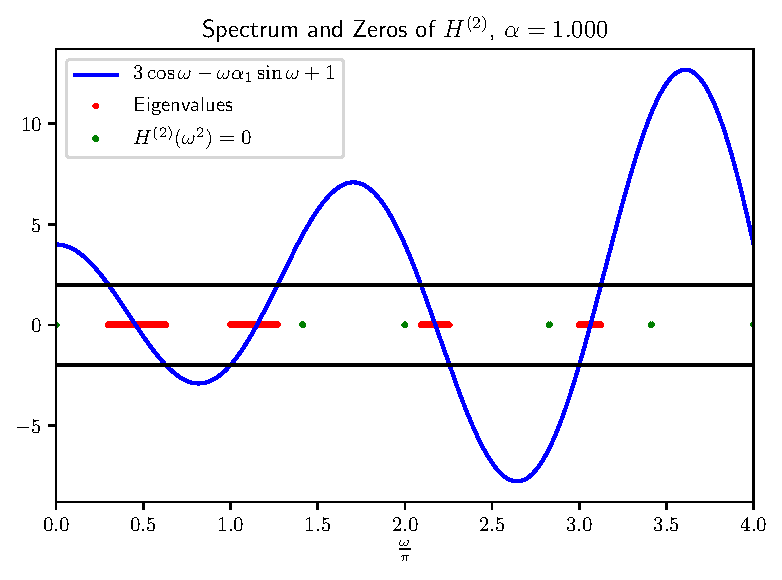
\includegraphics[scale=0.55]{1DDecoratedGraph_alpha1.pdf}
		\caption{\label{fig:1DDecoratedGraph_alpha1} The values of $\omega$ which solve \eqref{eq:EmbeddedGraphDetSolveCondition} with $\alpha_1=1$. No zeros of $H^{(2)}$ form part of the spectrum in this case.}
	\end{subfigure}
	~
	\begin{subfigure}[t]{0.45\textwidth}
		\centering
		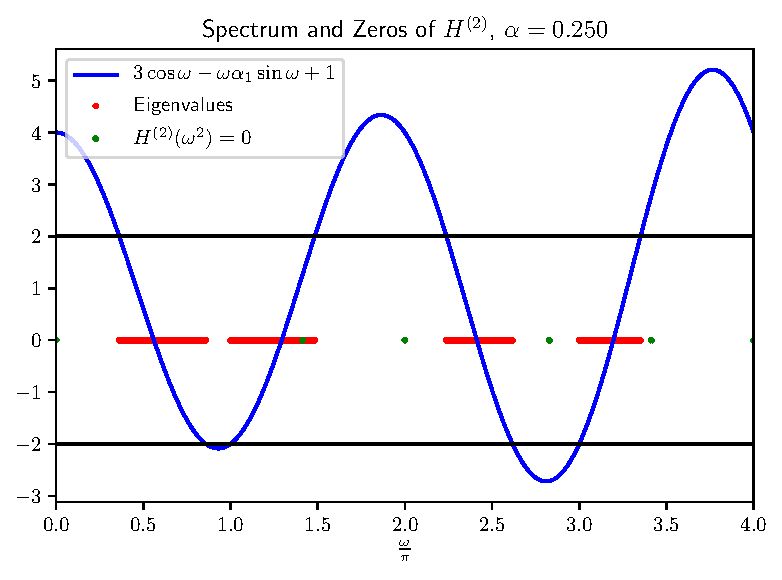
\includegraphics[scale=0.55]{1DDecoratedGraph_alpha0-25.pdf}
		\caption{\label{fig:1DDecoratedGraph_alpha0-25} The values of $\omega$ which solve \eqref{eq:EmbeddedGraphDetSolveCondition} with $\alpha_1=\recip{4}$. With $\alpha_1$ this small, some of the zeros of $H^{(2)}$ form part of the spectrum.}
	\end{subfigure}
	\caption{\label{fig:1DDecoratedGraph} The values of $\omega$ which solve \eqref{eq:EmbeddedGraphDetSolveCondition}, using $a=\recip{\sqrt{2}}$. Changing the value of $\alpha$ effects how many zeros of $H^{(2)}$ are included in the spectrum. The ``Dispersion Relation" refers to the expression $3\cos\omega + \alpha\omega\sin\omega - 1$.}
\end{figure}
Zeros of $H^{(2)}$ occur at $\omega= 2n\pi, \frac{n\pi}{a}, \frac{n\pi}{b}$, which also solve \eqref{eq:EmbeddedGraphDetSolveCondition} for all values of $\qm$.
Examining the limit \eqref{eq:EigenvalueBranchLimit} reveals that a zero of $H^{(2)}$, say $\omega_0$, is part of the spectrum only when there exists a $\qm_0\in\left[-\pi,\pi\right)$ such that $\Xi\bracs{\omega_0}=\cos\theta_0+\recip{2}$.
That is, the bracketed term in \eqref{eq:EmbeddedGraphDetSolveCondition} is required to be zero for a root of $H^{(2)}$ to be part of the spectrum.
The eigenvalue branches in the vicinity of root $\omega_0=\pi\sqrt{2}$ are plotted in figure \ref{fig:1DDecoratedGraphEvalBranches-Thetas}, to illustrate this point.
\begin{figure}[t!]
	\centering
	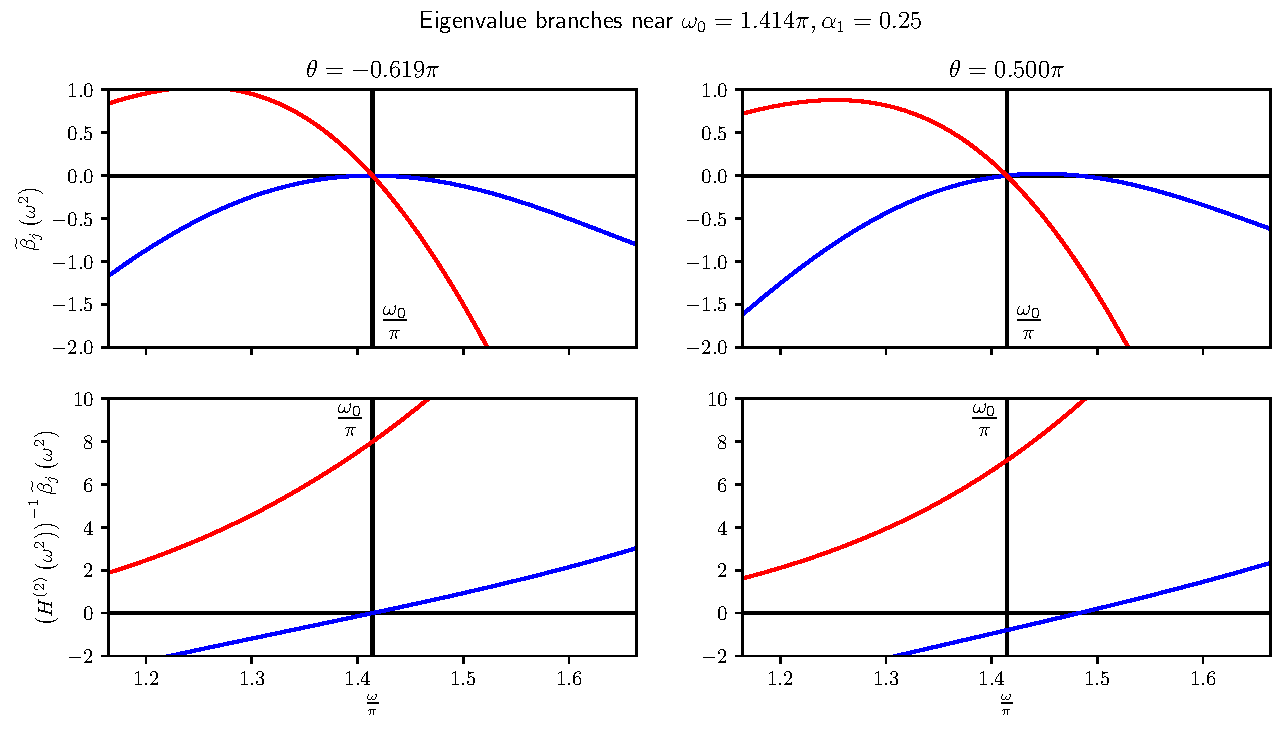
\includegraphics[scale=0.7]{1DDecoratedGraphEvalBranches-Thetas.pdf}
	\caption{\label{fig:1DDecoratedGraphEvalBranches-Thetas} eigenvalue branches of the matrix $\mathfrak{M}_{\qm}$ near $\omega_0 = \pi\sqrt{2}$, which is a root of $H^{(2)}$. The value $\qm_0\approx-0.691\pi$ solves $\Xi\bracs{\omega_0}=\cos\qm_0+\recip{2}$, and the limit \eqref{eq:EigenvalueBranchLimit} is zero. At other values of $\qm$ however, the limit \eqref{eq:EigenvalueBranchLimit} is non-zero.}
\end{figure}
It is also worth noting that (in figure \ref{fig:1DDecoratedGraphEvalBranches-Thetas}) there are two eigenvalue branches which are zero at $\omega_0$, with the third being non-zero at $\omega_0$.
For both branches, the limit \eqref{eq:EigenvalueBranchLimit} exists, however only for one is it zero.
The spectrum of \eqref{eq:WholeSpaceLaplaceEqn} thus consists of those $\omega$ such that
\begin{align*}
	\abs{ 3\cos\omega + \alpha\omega\sin\omega - 1 } \leq 2.
\end{align*}
As expected, the spectrum does not depend on $\beta$ despite the fact that the $M$-matrix for each operator on $\graph_{\mathcal{P}}$ does.
It does differ from the spectrum of the quantum graph in section \ref{ssec:Example1DLoop} due to the presence of the ``decoration" $I_{12}$, although this difference only depends on the length of the additional edge $I_{12}$.

\subsection{Cross in the Periodic Plane} \label{ssec:ExampleCrossInPlane}
Our final example is a two-dimensional graph whose period cell represents a lattice-like structure in $\reals^2$.
Consider the embedded, periodic graph defined as follows --- for each $\bracs{n,m}\in\integers^2$ define
\begin{align*}
	v^{(n,m)} &= \bracs{n+\recip{2}, m+\recip{2}}, \quad
	I_{\mathrm{left}}^{\bracs{n,m}} = \sqbracs{v^{\bracs{n,m}}, v^{\bracs{n+1,m}}}, \quad
	I_{\mathrm{up}}^{\bracs{n,m}} = \sqbracs{v^{\bracs{n,m}}, v^{\bracs{n,m+1}}}, \\
	\vertSet^* &= \clbracs{v^{\bracs{n,m}} \setVert \bracs{n,m}\in\integers^2}, \quad
	\edgeSet^* = \clbracs{ I_{\mathrm{l}}^{\bracs{n,m}}, I_{\mathrm{u}}^{\bracs{n,m}} \setVert \bracs{n,m}\in\integers^2}, \quad
	\graph^* = \bracs{\vertSet^*, \edgeSet^*}.
\end{align*}
Place a coupling constant $\alpha^{\bracs{n,m}} =: \alpha_3>0$ at each $v^{(n,m)}$.
The period graph of $\graph^*$ occupies $\left[0,1\right)^2$ and consists of a single vertex with two looping edges of length 1.
Breaking the loops by introducing two artificial vertices takes us to the quantum graph
\begin{align*}
	\vertSet = \clbracs{v_1, v_2, v_3}, \quad
	\edgeSet = \clbracs{I_{13}, I_{31}, I_{23}, I_{32}}, \quad
	\graph = \bracs{\vertSet, \edgeSet},
\end{align*}
with
\begin{align*}
	l_{13} = b, \quad l_{31} = \tilde{b} := 1-b, \quad 
	l_{23} = a, \quad l_{32} = \tilde{a} := 1-a, \qquad
	\qm_{13} = \qm_{31} = \qm_2, \quad \qm_{23} = \qm_{32} = \qm_1,
\end{align*}
and coupling constant $\alpha_3$ at $v_3$ (and zero coupling constants at the dummy vertices $v_1$ and $v_2$).
To avoid notational clutter, we also define
\begin{align*}
	s_a &= \sin\bracs{a\omega}, \quad 
	c_a = \cos\bracs{a\omega}, \quad 
	s_b = \sin\bracs{b\omega}, \quad 
	c_b = \cos\bracs{b\omega}, \\
	\tilde{s}_a &= \sin\bracs{\omega\bracs{1-a}}, \quad 
	\tilde{c}_a = \cos\bracs{\omega\bracs{1-a}}, \quad 
	\tilde{s}_b = \sin\bracs{\omega\bracs{1-b}}, \quad 
	\tilde{c}_b = \cos\bracs{\omega\bracs{1-b}}.
\end{align*}
Using corollary \ref{cory:M-MatrixEntriesNoPoles} we set $H^{(2)} = s_a s_b \tilde{s}_a \tilde{s}_b$, and obtain
\begin{align*}
	\mathfrak{M}_{\qm} &=
	\begin{pmatrix}[2.5]
		-\omega s_a \tilde{s}_a \bracs{ s_b \tilde{c}_b + c_b \tilde{s}_b } &
		0 &
		\begin{split}
			&\omega s_a \tilde{s}_a \bracs{ e^{\rmi\qm_2\tilde{b}}s_b + e^{-\rmi\qm_2 b}\tilde{s}_b }
		\end{split} \\
		0 &
		-\omega s_b \tilde{s}_b \bracs{ s_a \tilde{c}_a + c_a \tilde{s}_a } &
		\begin{split}
			&\omega s_b \tilde{s}_b \bracs{ e^{\rmi\qm_1\tilde{a}}s_a + e^{-\rmi\qm_1 a}\tilde{s}_a } 
		\end{split} \\
		\omega s_a \tilde{s}_a \bracs{ e^{-\rmi\qm_2\tilde{b})}s_b + e^{\rmi\qm_2 b}\tilde{s}_b } &
		\omega s_b \tilde{s}_b \bracs{ e^{-\rmi\qm_1\tilde{a}}s_a + e^{\rmi\qm_1 a}\tilde{s}_a } &
		\begin{split}
			&-\omega ( s_a s_b \tilde{s}_a \tilde{c}_b 
			+ s_a s_b \tilde{c}_a \tilde{s}_b \\ 
			& + s_a c_b \tilde{s}_a \tilde{s}_b
			+ c_a s_b \tilde{s}_a \tilde{s}_b \\
			& - \omega\alpha_3 s_a s_b \tilde{s}_a \tilde{s}_b )
		\end{split}
	\end{pmatrix}.
\end{align*}
Examining \eqref{eq:QGDetSolveCondition} yields
\begin{align} \label{eq:ExampleThickVertexSolution}
	0 = \omega^3 s_a^2 s_b^2 \tilde{s}_a^2 \tilde{s}_b^2 \sin\bracs{\omega} 
	\bracs{ 4\cos\bracs{\frac{\qm_1+\qm_2}{2}}\cos\bracs{\frac{\qm_1-\qm_2}{2}} + \omega\alpha_3\sin\omega - 4\cos\omega}.
\end{align}
For ease, we define
\begin{align*}
	\Xi\bracs{\omega} := \cos\omega - \frac{\alpha_3\omega}{4}\sin\omega.
\end{align*}
From here, the analysis is similar to that of example \ref{ssec:EmbeddingDependentExample} --- any root of $H^{(2)}$ solves \eqref{eq:ExampleThickVertexSolution}, in addition to those $\omega$ for which $-1\leq\Xi\bracs{\omega}\leq 1$.
Examination of the eigenvalue branches then produces a familiar conclusion; a root of $H^{(2)}$, say $\omega_0$, forms part of the spectrum of \eqref{eq:QGFullSystem} on $\graph$ if and only if there exists a $\qm_0$ such that the bracket in \eqref{eq:EmbeddedGraphDetSolveCondition} is zero at $\bracs{\omega_0,\qm_0}$.
As a result, the spectrum consists of exactly those $\omega$ such that
\begin{align*}
	-1 \leq \cos\omega - \frac{\alpha_3\omega}{4}\sin\omega \leq 1.
\end{align*}
To round off the analysis, quantities such as the integrated density of states (IDoS) and density of states (DoS) can also be estimated from \eqref{eq:ExampleThickVertexSolution}, which demonstrating that the spectrum ``concentrates" at the center of each spectral band.
Examples are shown in figure \ref{fig:CrossInPlane_ScalarDoS}.
\begin{figure}[b!]
	\begin{subfigure}[t]{0.45\textwidth}
		\centering
		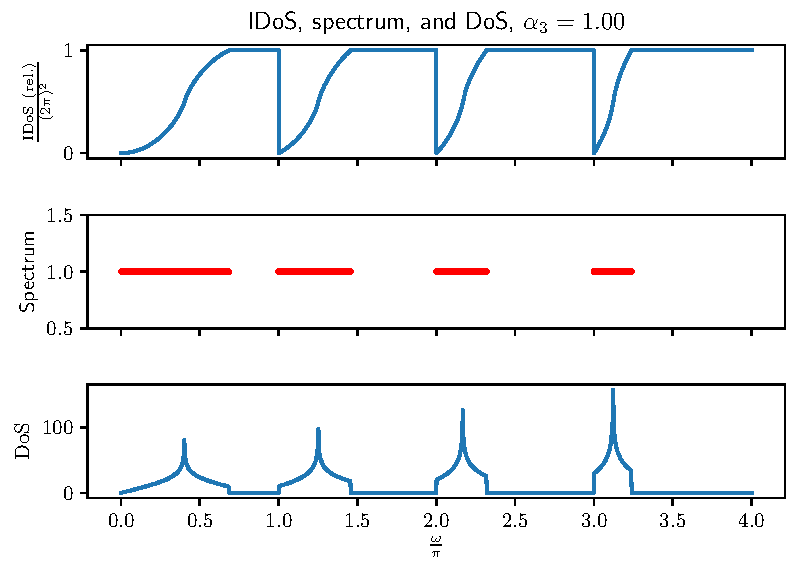
\includegraphics[scale=0.5]{CrossInPlane_ScalarDoS_alpha1-00.pdf}
		\caption{\label{fig:CrossInPlane_ScalarDoS_alpha1-00} The (relative) integrated density of states (IDoS), density of states (DoS) and spectrum for the system with $\alpha_3=1$.}
	\end{subfigure}
	~
	\begin{subfigure}[t]{0.45\textwidth}
		\centering
		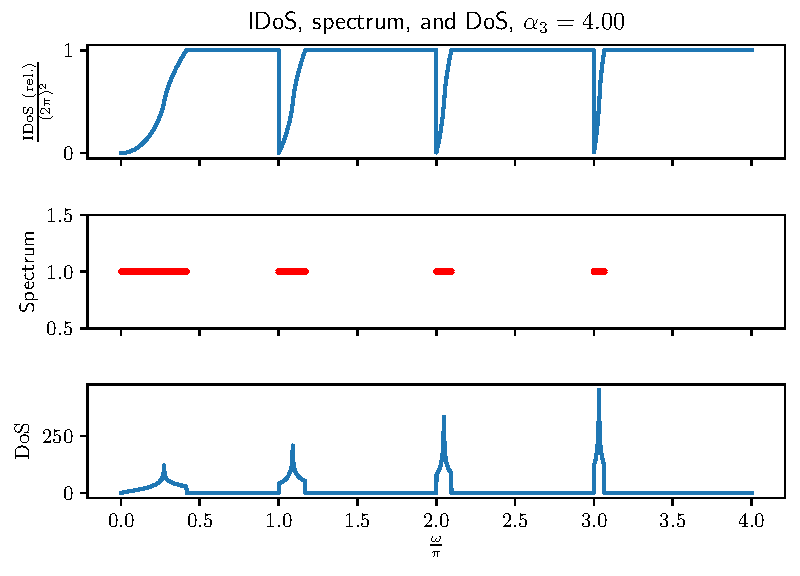
\includegraphics[scale=0.5]{CrossInPlane_ScalarDoS_alpha4-00.pdf}
		\caption{\label{fig:CrossInPlane_ScalarDoS_alpha4-00} The (relative) integrated density of states (IDoS), density of states (DoS) and spectrum for the system with $\alpha_3=4$.}
	\end{subfigure}	
	\caption{\label{fig:CrossInPlane_ScalarDoS} The (relative) IDoS, DoS, and spectrum for the graph topology in section \ref{ssec:ExampleCrossInPlane}.
	The relative IDoS at the value $x$ is defined as the IDoS at the value $x$ minus $\left\lfloor\frac{x}{\pi}\right\rfloor\bracs{2\pi}^2$.}
\end{figure}
For any $\alpha_3>0$, the spectrum comprises a union of pairwise disjoint ``spectral bands" $I_n\subset\sqbracs{(n-1)\pi, n\pi}$, each with left-endpoint $(n-1)\pi$ and a right-endpoint strictly less than $n\pi$.
It is worth remarking that this behaviour is reversed for $\alpha_3<0$, the bands having right-endpoint $n\pi$ and left-endpoint strictly greater than $(n-1)\pi$.
For $\alpha\leq-2$ there is even a gap between an isolated eigenvalue at $0$ and the beginning of the band $I_1$ --- however $\alpha<0$ breaks real-world constraints \tstk{should link back to where (if ANYWHERE) we mentioned thin-structure limit stuff?}.
This is consistent with similar applications of singular-structures as approximations to thin-material structures, like the work of \cite{cherednichenko2019time}, in which the natural physical constraints on the parameters in the problem prevent the opening of a band-gap at the bottom of the spectrum.


\chapter{Conclusion} \label{ch:Conclusion}
In this chapter we review the content of this report and speculate on the future direction of research.
Section \ref{sec:ConcTheory} will provide an overview of the existing theory that we have utilised, the motivation for our project and restate our research objectives.
We will then summarise the work we have done to build on this theory and towards these objectives in section \ref{sec:ConcWork}.
Finally, in section \ref{sec:ConcFuture} we shall discuss some of the loose ends or open questions that have been raised by our research or not yet addressed, and provide some direction for future work.

\section{Summary of Motivation, Research Objectives, and Existing Theory} \label{sec:ConcTheory}
Our research is motivated by applications to PCFs (section \ref{sec:ProjectMotivation}), specifically in investigating the nature how spectral band-gaps emerge due as a result of the geometries of the fibres.
Although our research centres on singular-structure problems as a starting point (section \ref{sec:OurPhysicalSetup}), there is a link through quantum graph problems back to familiar thin-structure problems that are commonly used model PCFs (section \ref{sec:GraphLitReview}).
This amounts to us being able to view our singular-structure problems in an intuitive manner - as the limit of thin-structure problems as the thickness of the structures tends to zero, although the manner in which this thickness tends to zero also influences the problems that we should be considering (section \ref{sec:GraphLitReview}).
As such, the research goals that we set out to achieve were:
\begin{enumerate}
	\item To demonstrate that the singular-structure problems we consider give rise to equivalent quantum graph problems, in turn linking our singular-structure problems to formal ``limits" of thin-structure problems and hence PCF models.
	\item To study singular-structure problems that can be seen as approximations to PCFs; deriving the equivalent quantum graph problems and providing insight into how the geometry of the fibre cross section influences the spectral band-gaps of the fibre.
	\item To propose numerical approaches to determining these band-gaps in the event that an analytic approach proves unfeasible.
\end{enumerate}

As we discussed in sections \ref{sec:VariationalProblemLitReview}, choosing to study singular-structure problems required us to rethink the concepts of gradient, curl and divergence.
This bought us to the theory of chapter \ref{ch:ScalarEqns}, in which we presented a framework for posing variational problems with respect to Borel measures and reviewed the existing theory on the matter.
We also provided a geometric insight into what the concept of gradient meant in the context of our singular-structure problems, and demonstrated how we could obtain an equivalent quantum graph problem from a variational problem.
These arguments formed the basis of our understanding and direction for our work in chapter \ref{ch:VectorEqns}. \newline

Quantum graph problems are comparatively well studied, there even being a comprehensive introductory text on the subject and a recent spike in research interest (section \ref{sec:GraphLitReview}).
As such we simply needed to borrow the relevant concepts and tools from the existing works in the area for our own purposes, which we did in chapter \ref{ch:QuantumGraphs}.
Of particular importance was the M-matrix and it's utility in solving spectral problems on quantum graphs; and we briefly touched on how the M-matrix opens these spectral problems up to numerical schemes in chapter \ref{ch:ExampleSystems}, a topic which we revisit in section \ref{sec:ConcFuture}.
We also use quantum graphs as the link between our singular-structure problems and thin-structure problems that describe PCFs.

\section{Summary of Work and Examples} \label{sec:ConcWork}
The work of chapter \ref{ch:VectorEqns} see us build on the existing work on variational problems by constructing the spaces $\ktgradSob{\ddom}{\ddmes}$, $\ktcurlSob{\ddom}{\ddmes}$ and $\ktcurlSobDivFree{\ddom}{\ddmes}$ and analysing the operator $\ktgrad$.
We provide an interpretation for the $\ddmes$-curl of a vector field (section \ref{sec:CurlExamples}) and also prove various properties about the elements of the aforementioned spaces.
In particular we deduce the form of the tangential $\kt$-curl and $\kt$-gradient, and characterise what it means to be divergence-free.
We also prove that the space $\ktcurlSob{\ddom}{\ddmes}$ has some inherent structural properties that are not obvious from it's construction (section \ref{sec:ktcurlSobExtraProperties}).
This analysis allows us to consider the singular-structure analogue of the ``curl-of-the-curl" equation, written in \eqref{eq:CurlCurlEquationDivFree} and determine the equivalent quantum graph problem in section \ref{sec:CurlReductionToQG}, forming the basis for our examples in chapter \ref{ch:ExampleSystems}.
This theory is essential if we are to address the first of our research objectives, as without knowledge of the form of objects like $\ktcurl{\ddmes}u$, we have no hope of obtaining an equivalent quantum graph problem from our singular-structure problems.
The fact that we can write problems like \eqref{eq:CurlCurlEquationDivFree} in the way they are presented is also satisfying in an intuitive sense; the ``equations" that we are studying have the same form as those which we would consider in the thin-structure setting, only now we have a different understanding of gradients (and curls, and divergences).
Our development of this theory will likely prove valuable if we are to move on from the ``curl-of-the-curl" equation to a full Maxwell problem involving coupled $\mathbf{E}$ and $\mathbf{H}$ fields, which we revisit in section \ref{sec:ConcFuture}. \newline

Having derived the equivalent quantum graph problem from our singular-structure problems, we spend chapter \ref{ch:ExampleSystems} looking over some examples and addressing the second and third objectives.
Our examples demonstrate how to construct the M-matrix, and how it can be used either analytically or numerically to solve spectral problems and hence reveal insights about band-gaps.
We take a mixture of numerical and analytic approaches in these examples, however stop short of a fully-fledged numerical scheme that begins from the M-matrix itself.
This is discussed in section \ref{sec:NumericalMethodsDiscussion} however, and will be revisited in section \ref{sec:ConcFuture}, which follows.
The examples also illustrate how it is possible to use the geometry of the cross-sectional structure to open band-gaps in the spectrum (section \ref{sec:ExampleGeneralLengths}).
However our investigation is limited to a single, simplified case and analytic progress proves hard, again highlighting that, at least for practical purposes, a numerical scheme that focuses on a physically relevant part of the spectrum may be more useful and applicable.
We provide a final example in section \ref{sec:ExampleThickVertex} that retains the geometry of the example in section \ref{sec:ExampleCrossInPlane}, but with a non-zero coupling constant at the central vertex.
The corresponding singular-structure problem corresponds to a different scaling limit (section \ref{sec:GraphLitReview}) than the previous examples, and in this case we demonstrate that band-gaps are opened simply by the presence of this coupling constant.
This in turn would suggest that thin-structures that adhere to this scaling between ``edge"- and ``vertex"-regions are more likely to give rise to band-gaps, however more work needs to be done beyond this example.
We make this suggestion because these examples demonstrate that the addition of a non-zero coupling constant can lead to the opening of band-gaps, however this may again be an artefact of the geometry of the problem rather than a general principle.
Another thing to be noted is that the M-matrix can be recycled from the first example, and the only difference in our solution method being that we consider a slightly different eigenvalue problem.
This is potentially useful for any numerical schemes - we only need construct (a function that evaluates) the M-matrix once for a given geometry (and set of governing equations).
If in addition we can produce results like proposition \ref{prop:M-MatrixEntries} for each quantum graph problem, there is the potential to further cut the complexity of such numerical constructions. \newline

Whilst our examples help us explore the second and third objectives, and do provide us with some intuition about what to expect, they do not provide us with any general insights yet.
This, alongside some of the considerations for a numerical scheme, are discussed in section \ref{sec:ConcFuture}.

\section{Further Developments} \label{sec:ConcFuture}
The work that has been carried out thus far makes progress towards the research objectives that were set out in section \ref{sec:ReportOverview}, but stops short of providing definitive answers in places.
In this section we examine some of these loose ends, and the direction of future work that could be undertaken to address them.
We cover issues surrounding a numerical scheme for solving our singular-structure problems in section \ref{sec:ConcFutureNumerical}; how we might look to qualify the dependence of the graph geometry on the spectrum of our problems in section \ref{sec:ConcFutureGeometry}, and discuss how we might make progress onto modelling electromagnetic wave-guidance through Maxwell's equations in section \ref{sec:ConcFutureMaxwell}.
Once we have explored these issues, we will conclude with section \ref{sec:ConcClosingRemarks}.

\subsection{Considerations for Numerical Schemes} \label{sec:ConcFutureNumerical}
In section \ref{sec:NumericalMethodsDiscussion} we discussed the possibility of using the M-matrix to explore the spectrum of quantum graph (hence our singular-structure) problems numerically.
Here we review what was said and elaborate on how such an approach might be developed, tested and analysed.
To make the discussion as general as possible; in this section we assume that we have some family of quantum graph problems $\mathcal{P}_{\qm}$, with spectral parameter $\lambda$ and spectra $\sigma\bracs{\mathcal{P}_{\qm}}$, each having an M-matrix $M_{\qm}\bracs{\lambda}$.
This family $\mathcal{P}_{\qm}$ is the result of taking a Gelfand transform of a periodic quantum graph problem $\mathcal{P}$ (with spectrum $\sigma\bracs{\mathcal{P}}$), that is equivalent to some singular-structure problem that we are concerned with.
Here we discuss a numerical scheme that is capable of being told the problems $\mathcal{P}_{\qm}$ and producing an approximation to the spectrum of $\mathcal{P}$, whose outline is along the lines of the following;
\begin{enumerate}
	\item Consider the spectral problem $\mathcal{P}_{\qm}$ as a generalised eigenvalue problem
	\begin{align*}
		M_{\qm}\bracs{\lambda} v &= 0,
	\end{align*}
	involving the M-matrix.
	\item Determine a method for constructing $M_{\qm}\bracs{\lambda}$.
	\item Solve the generalised eigenvalue problem $\mathcal{P}_{\qm}$ for $\sigma\bracs{\mathcal{P}_{\qm}}$, and hence construct an approximation to the spectrum of $\mathcal{P}$.
\end{enumerate}
Broadly speaking; the issues surround how to construct the M-matrix efficiently and quickly, and the optimal method of determining the spectrum of $\mathcal{P}_{\qm}$ and hence $\mathcal{P}$.
We discuss each of these below, along with how they might be addressed. \newline

\subsubsection{Construction of the M-Matrix} \label{sec:ConcFutureConstructM}
Any numerical scheme will require a method for constructing the M-matrix, because the solver for the generalised eigenvalue problem will need this ability.
Naively we can construct the M-matrix simply by following the constructive proof of proposition \ref{prop:MMatrixEntries} numerically, for each value of $\lambda$ that we are required to evaluate $M_{\qm}$ at.
This involves solving each edge-ODE in $\mathcal{P}_{\qm}$ numerically, and once for each column of the M-matrix (although this is a large overestimate and can be reduced - see section \ref{sec:NumericalMethodsDiscussion}), reading off the approximate Neumann data for the edge solution, and then summing the appropriate combination of derivatives at the vertices.
Needless to say this will be an expensive process for a large (in the sense of number of edges) graph, given that it needs to be done each time the M-matrix needs to be evaluated.
Having said this we should also note that this method is relatively simple to program, and provided there was sufficient care in solving the edge-ODEs of $\mathcal{P}_{\qm}$ would provide access to the M-matrix. \newline

We can make constructing the M-matrix cheaper (in computational terms) by employing one of the tactics in chapter \ref{ch:ExampleSystems} - working analytically to a suitable point and then proceeding numerically when the expressions become too complex.
The obvious candidate for a stopping point for each $\mathcal{P}_{\qm}$ would be the analogue of proposition \ref{prop:M-MatrixEntries}, as this bypasses the need to solve each edge-ODE every time the M-matrix needs to be evaluated (and even provides the M-matrix as a function of $\lambda=\omega^2$ and the quasi-momentum $\qm$).
In fact this result reduces the construction of the M-matrix to a case of looking up geometric properties of the underlying graph and evaluating trigonometric functions.
Of course the exchange we make for this simpler construction of $M_{\qm}$ is that we loose generality in our numerical scheme; proposition \ref{prop:M-MatrixEntries} only holds for the specific set of equations we chose to examine in chapter \ref{ch:ExampleSystems}, and so we would have to prove an analogue of proposition \ref{prop:M-MatrixEntries} for each quantum graph problem we want to consider. \newline

At present, computer code is being developed to construct the M-matrix for the set of equations \eqref{eq:QGEquation} using proposition \ref{prop:M-MatrixEntries}, and we will also be looking to write code for the more general approach that relies on solving the edge-ODEs directly.
However the bottom line of this issue is that future work needs to be done looking into the computational cost and accuracy of both approaches.
For the purely numerical approach the direction of research is fairly clear; we should look at existing theory in this area that surrounds the ODE solvers that we would be employing, and couple this with the algorithm that we end up proposing to construct the M-matrix.
The alternative approach requires slightly different treatment, as although in theory one will obtain exact expressions for the elements of the M-matrix, we do not yet know how easy it will be to obtain an analogue of proposition \ref{prop:M-MatrixEntries} when the edge-ODEs of $\mathcal{P}_{\qm}$ change.
Indeed it may not even be possible to obtain such a result, or the end-user of the numerical scheme may not want to spend time deriving it.
Assuming we have such a result however, we can do some basic analysis on the computational cost of assembling the M-matrix using this approach and then compare this with the alternative approach.
Although we expect the latter (analytic entries) approach to be more accurate and faster in all situations, the extent of these gains might be considered too small to warrant the derivation of an analogue of proposition \ref{prop:M-MatrixEntries}.

\subsubsection{Determination of the Spectrum of $\mathcal{P}$} \label{sec:ConcFutureGetSpectrum}
The other consideration for our numerical scheme are the nuances that come with solving the generalised eigenvalue problems, and how we construct an approximation to $\sigma\bracs{\mathcal{P}}$ from the values we get for $\sigma\bracs{\mathcal{P}_{\qm}}$.
The foremost problems with the latter is that we cannot take the union of each of the spectra $\sigma\bracs{\mathcal{P}_{\qm}}$ over the $\qm$ as we did analytically - we will be forced to (at best) use a fine mesh of discrete $\qm$ values to build up an approximation to $\sigma\bracs{\mathcal{P}}$.
As such one glaring issue is whether we can quantify how fine a mesh in $\qm$ is required, or whether there are certain values of $\qm$ that are of significance to the spectrum (values that correspond to eigenvalues found at the ends of band-gaps, for example).
There may also be symmetries that we can exploit on a problem-by-problem basis; like in the example in section \ref{sec:ExampleCrossInPlane} where there was symmetry in the components of $\qm$ and hence we could set $\qm_2=0$ to determine the spectrum.
However if we expect some kind of stability of $\sigma\bracs{\mathcal{P}_{\qm}}$ with respect to $\qm$ (that is, we can show that small changes in $\qm$ correspond to some kind of small changes in $\sigma\bracs{\mathcal{P}_{\qm}}$) then the idea of meshing $\qm$ and solving a finite number of the $\mathcal{P}_{\qm}$ isn't a terrible one.
Given the lack of immediate alternative suggestions, this kind of analysis is the way to go on this front. \newline

The former problem mentioned above, the nuances that come with solving the generalised eigenvalue problems, are another concern.
In particular we have to deal with the complication that there may be (and in our case will almost always be) an infinite number of solutions $\bracs{\lambda,v}$ to $M_{\qm}\bracs{\lambda} v = 0$.
Some knowledge of the form of the M-matrix (like proposition \ref{prop:M-MatrixEntries}) is helpful in this regard, for example we know that if the M-matrix is periodic in $\lambda$ then it is sufficient to determine all the unique eigenvalues over one period and from there can construct the remainder.
However even if the M-matrix is periodic the presence of coupling constants on the vertices can make this potential advantage redundant, as can be seen for the M-matrix of section \ref{sec:ExampleThickVertex}.
If a numerical scheme is being used solely from a fabrication/design perspective, then there is always the option to restrict the solver to finding eigenvalues $\lambda$ within a given range of interest, such as the operating frequencies of a PCF in the electromagnetic setting.
We should also not forget that, regardless of the computational power available to us, we can never determine the full spectrum computationally either (we require some analytic techniques for this) and so this compromise is likely one of the best we can provide.
This in turn raises a further question - given a particular range of interest for $\lambda$, how can be we be sure to find every eigenvalue in $\sigma\bracs{\mathcal{P}_{\qm}}$ that lies in this range?
An examination of existing solver methods for generalised eigenvalue problems would go some way to answering this question, alongside whether we can deduce (analytically) anything about the distribution of the eigenvalues for a given $\mathcal{P}_{\qm}$.

\subsection{Effect of Geometry on Spectra} \label{sec:ConcFutureGeometry}
One of our objectives was to attempt to describe how the underlying geometry of the singular-structure affects the resulting spectrum and hand-gaps that the structure exhibits, and some progress has been made with this through the theory of chapter \ref{ch:VectorEqns}.
Namely we see that the $\qm$ undergoes rotations dependant on the orientations of the underlying graph and the quantum graph problem that we obtain has solutions dependant on the lengths of the singular-structure edges.
And although we have not provided the details; it is also known that the relative scaling of the vertex- and edge-regions in the thin-structures we are approximating gives rise to different quantum graph problems and hence different spectra, as we illustrated in the examples of section \ref{sec:ExampleCrossInPlane} and \ref{sec:ExampleThickVertex}.
By affecting the coupling constants (through the scaling of the micro-structure), quasi-momentum and incorporating the edge-lengths, the spectrum and hence band-gaps of the structure are also changed.
This being said, we have not drawn any general insights into how these effects change the resulting spectra, only provided examples in chapter \ref{ch:ExampleSystems} to demonstrate that they do.
We can make one conjecture on this topic though; that a graph with zero coupling constants and (geometric) symmetry in the periodic directions will not give rise to band-gaps.
This idea is reinforced by the examples of section \ref{sec:ExampleCrossInPlane} and \ref{sec:ExampleGeneralLengths}, as well as other examples with geometric symmetries that we have looked at but didn't include in this report. \newline

Another consideration that goes beyond what we have done in this report is looking at geometries whose peroid-cells are not rectangular in shape.
This direction of future work is motivated more by the desire to produce a model that is relevant to physical PCFs and wave-guidance problems, rather than mathematical interest or completeness.
In particular PCFs are typically fabricated with hexagonal lattice-structures, which for us would result in a hexagonal unit cell for our infinite, periodic singular-structure.
The affect is largely felt by the Gelfand transform, as we no longer have a set of orthogonal vectors that describe the translation-invariance of the singular-structure.
We expect the analysis we have carried out in chapter \ref{ch:VectorEqns} to still be of relevance in this slightly altered case; in particular we have demonstrated that curls and gradients of zero are invariant with respect to the quasi-momentum, and so we expect that these objects will not change in these new period cell shapes.
Regardless, there is the option to investigate any changes that the shape of the period cell itself induces in the problems that we obtain, and the work in chapter \ref{ch:VectorEqns} can be used as a basis for this research.

\subsection{Generalisations to our Singular-Structure Systems} \label{sec:ConcFutureMaxwell}
We focused our attention on the ``curl-of-the-curl" equation \eqref{eq:CurlCurlDivFree} in chapters \ref{ch:VectorEqns} and \ref{ch:ExampleSystems} because it arises from the time-harmonic Maxwell system which describes electromagnetic wave propagation.
However the ``curl-of-the-curl" equation can only be derived if we assume a time-harmonic solution to the full Maxwell system, namely assume that the $\mathbf{E}$ and $\mathbf{H}$ fields are of the form
\begin{align*}
	\mathbf{E}\bracs{x_1,x_2,x_3} = \widehat{\mathbf{E}}\bracs{x_1,x_2,x_3}e^{-i\omega t}, 
	&\quad  \mathbf{H}\bracs{x_1,x_2,x_3} = \widehat{\mathbf{H}}\bracs{x_1,x_2,x_3}e^{-i\omega t}.
\end{align*}
Substituting this ansatz into the system of Maxwell equations \eqref{eq:MaxwellSystem} and taking the curl of either equation and substituting the result into the other then provides the curl of the curl equation.
Whilst there is probably little harm in using the ``curl-of-the-curl" equation as our starting point for out singular-structure problems; for the purposes of providing a complete description of electromagnetic wave-guidance on singular-structures it would be good to derive an equivalent quantum graph problem for the system of Maxwell equations.
One could then use the quantum graph problem derived in chapter \ref{ch:VectorEqns} as a check for consistency in the system that was obtained.
No major obstacles are expected by from leaving the dependence on time in the system, however there will need to be some care in how to setup the various function spaces that we are working with.
However because the time co-ordinate is essentially separate from the spatial co-ordinates, we should be able to recycle the work in chapter \ref{ch:VectorEqns} here. \newline

Another possible generalisation that could be made to our systems concerns the ``empty space" (the cores if we adopt the language of PCFs) in our cross-sectional structure.
Currently our singular-structure problems effectively ignore this part of our domain, which lends itself to the description that there is no field $u$ in that part of the domain (or we don't care what it is).
In the context of electromagnetism this would likely mean that this ``empty space" was actually filled with a metallic material, and so we wouldn't expect a field in this region.
In reality this may not be the case (although metallic mode confinement in PCFs has been demonstrated, see \cite{hou2008metallic}), fibres are typically fabricated using two dielectric materials (one of which may be vacuum for PCFs).
As such we would need to consider the system of Maxwell equations \eqref{eq:MaxwellSystem} both on the singular-structure and in the remainder of the domain, and the electric permittivity $\eps_{P}$ and magnetic permeability $\mu_{P}$ would no longer be constant across the whole domain.
This opens up several avenues for exploration - foremost being how to correctly formulate Maxwell's equations in this instance.
We would be required to keep the variational approach we have adopted to deal with the singular-structure correctly, and so the natural avenue of investigation would be to adapt the measure that we pose our variational problem with respect to.
The foremost candidate being a ``Lebesgue plus singular graph" measure, namely a Borel measure
\begin{align*}
	\dddmes\bracs{B} &= \lambda_{2}\bracs{B} + \ddmes\bracs{B}, \quad B\in\mathcal{B}_{\ddom},
\end{align*}
where we now account for the singular structure using our singular measure on the underlying graph $\ddmes$ as before, but also add the standard 2D Lebesgue measure $\lambda_2$ so that we no longer discard the larger regions.
Again using a variational problem posed with respect to $\dddmes$ will allow us to deal with the issue of boundary conditions between the singular structure and surrounding dielectric, but whether we can determine a method to solve such problems (as we did by borrowing theory from quantum graphs) remains open.
There would also be similar questions raised about whether such a variational problem could still be thought of as the limit of some thin-structure problem, like with the singular-structure problems we have considered through this report thus far.

\section{Closing Remarks} \label{sec:ConcClosingRemarks}
The work in this report has made progress towards addressing the research objectives that it set out to achieve, as laid out in chapter \ref{ch:Intro}.
We look to consider singular-structure domains as setup in section \ref{sec:OurPhysicalSystem}, motivated by existing theory for variational problems (section \ref{se:VariationalProblemsLitReview}, chapter \ref{ch:ScalarEqns}) and seeking a consistent framework for our approximation to physical waveguides.
We develop this theory of variational problems in the context of our singular-structure problems in chapter \ref{ch:VectorEqns}; describing what the concepts of gradient, curl and divergence-free mean and hence building appropriate function spaces for our problems.
Furthermore, a link to quantum graph problems from our singular-structure problems is established (section \ref{sec:CurlReductionToQG}), meaning we can bring in existing theory from quantum graph problems (section \ref{sec:GraphLitReview}, chapter \ref{ch:QuantumGraphs}) to aid in the solution to our original singular-structure problems, and open up the potential for numerical approaches to be used (section \ref{sec:NumericalMethodsDiscussion}).
The link to quantum-graph problems also solidifies our singular-structure problems as formal limits of more familiar thin-structure models for waveguides (section \ref{sec:GraphLitReview}), addressing the first of the research objectives.
The examples of chapter \ref{ch:ExampleSystems} serves the purpose of bringing together the theory of the previous chapters and highlighting important considerations for solving our singular-structure problems.
We are able to demonstrate analytically that certain geometries (underlying graphs) give rise to band-gap spectra whilst others do not, and discuss how a numerical scheme that is designed to solve such problems might be employed (section \ref{sec:NumericalMethodsDiscussion}).
These examples also go some way to addressing research objectives two and three, although as we highlight in section \ref{sec:ConcFuture} there are further considerations and questions that need answering.
Section \ref{sec:ConcFutureMaxwell} also highlights that we have not yet fully addressed the first research objective, at least in the context of PCFs (electromagnetic wave-guidance) which is another direction we should pursue. \newline

In summary, the work presented in this report serves as a basis for future work on the objectives in chapter \ref{ch:Intro}.
The existing theory gathered, and that which has been developed, will allow further investigation into (limits of) more descriptive wave-guidance problems - addressing objective one.
The examples that have been analysed provide some underlying intuition about what we should expect the answers to objective two should be, and highlight the issues that a numerical scheme sought by objective three will need to consider.
We have discussed the direction of future work that will be taken with each of these objectives in mind throughout section \ref{sec:ConcFuture}, and will look to pursue these directions in the immediate future.

\newpage %have a new page to start the bibliography
\bibliographystyle{acm}
\bibliography{Paper_Scalar2020.bib}
\newpage %new page to clear space between bibliography and the appendix, as \section doesn't call \newpage

\section{Appendix} \label{sec:Appendix}

\end{document}